% ==========================
% Appendices
% ==========================

\section*{Appendix A: Survey Results}
\addcontentsline{toc}{section}{Appendix A: Survey Results}
\label{sec:appendix_a}

The following figures present the results of the requirements elicitation survey distributed to practising DevOps and Site Reliability Engineers. The survey comprised ten questions addressing current diagnostic pain points, acceptable response latency, confidence presentation preferences, and dashboard feature priorities.

\begin{figure}[H]
\centering
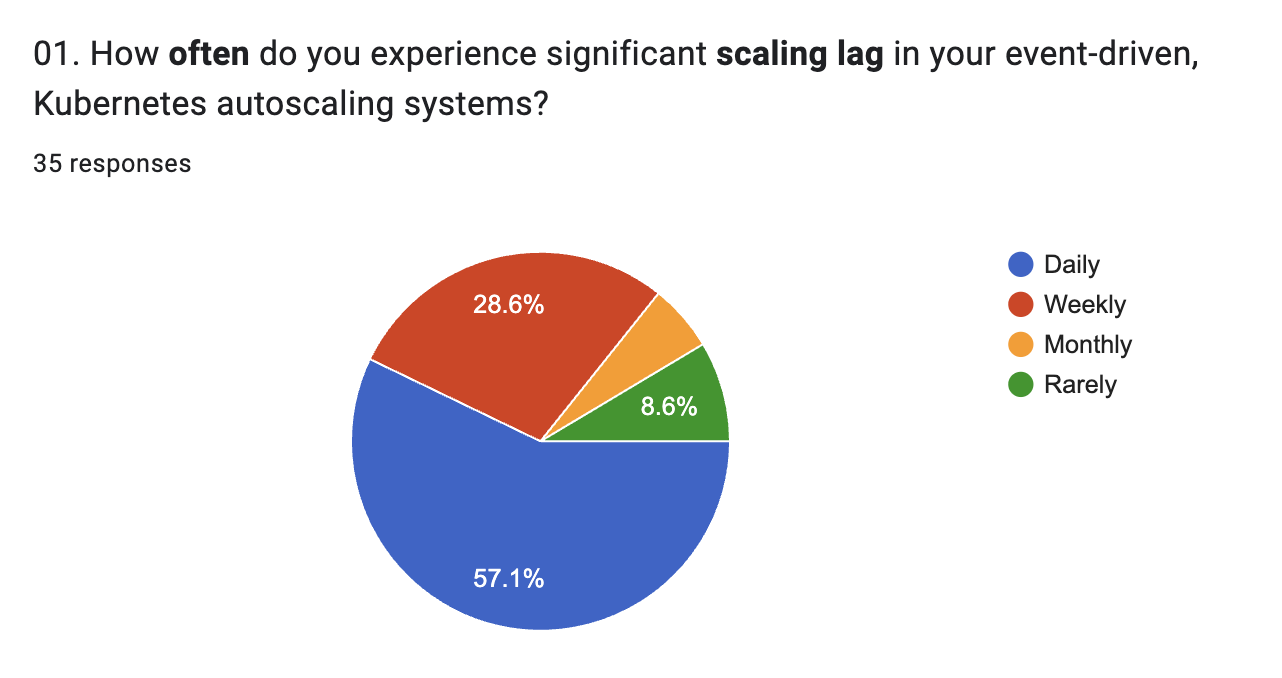
\includegraphics[width=\textwidth]{assets/survey/Q1.png}
\caption{Frequency of autoscaling delays encountered}
\label{fig:app_q1}
\end{figure}

\begin{figure}[H]
\centering
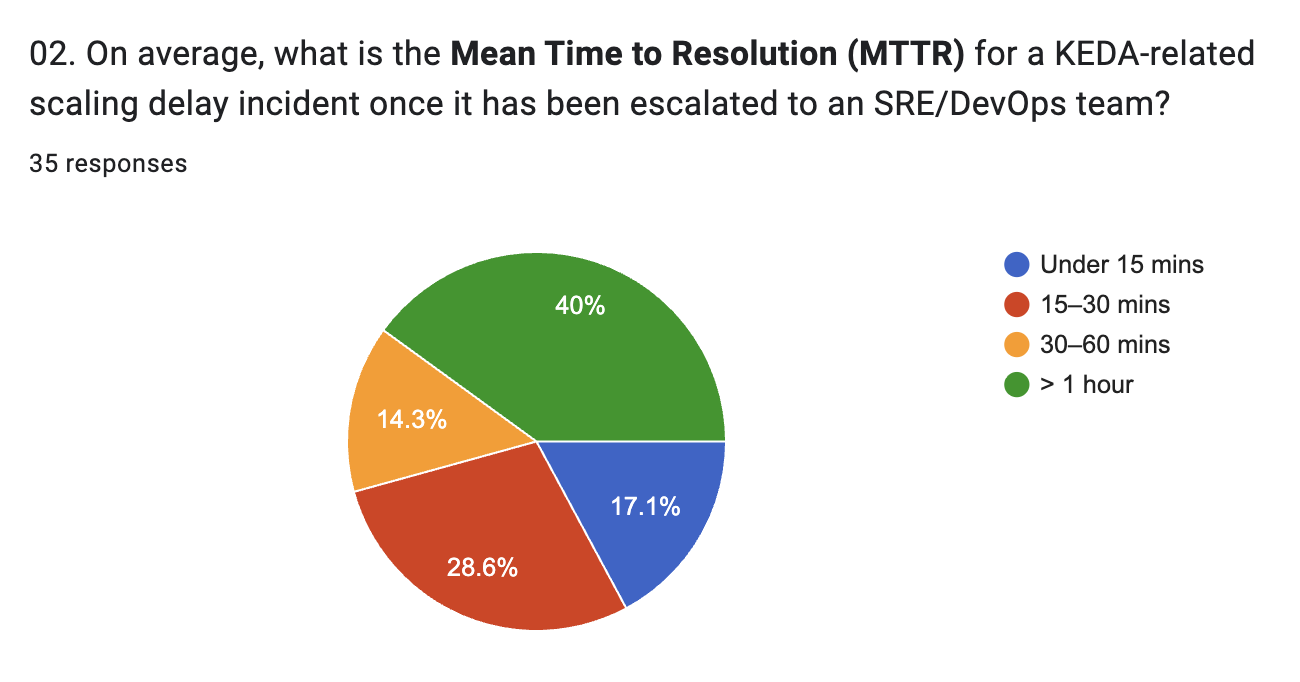
\includegraphics[width=\textwidth]{assets/survey/Q2.png}
\caption{Duration of manual root cause diagnosis}
\label{fig:app_q2}
\end{figure}

\begin{figure}[H]
\centering
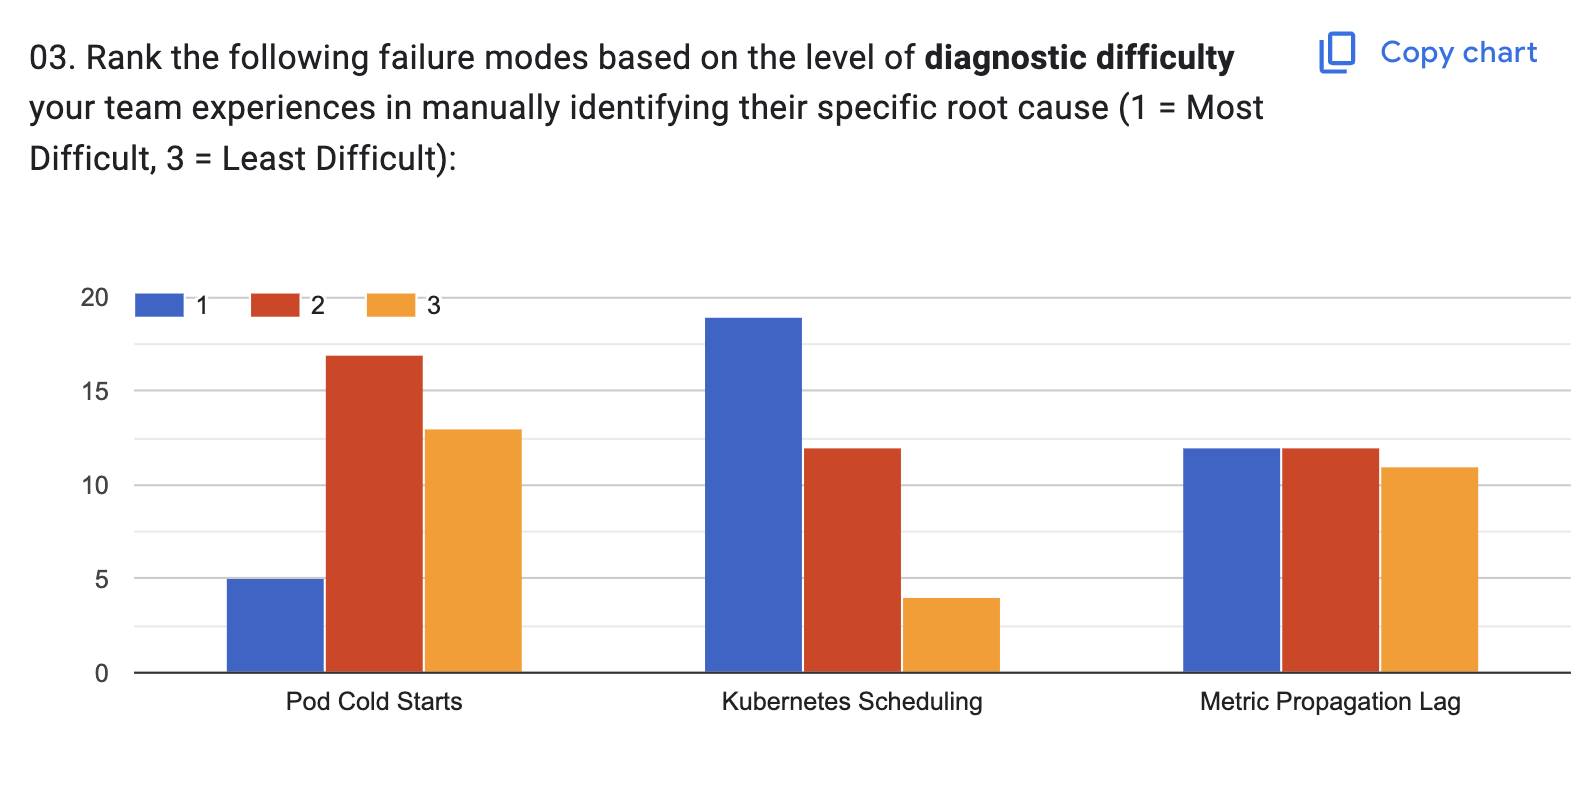
\includegraphics[width=\textwidth]{assets/survey/Q3.png}
\caption{Most frequently encountered root cause category}
\label{fig:app_q3}
\end{figure}

\begin{figure}[H]
\centering
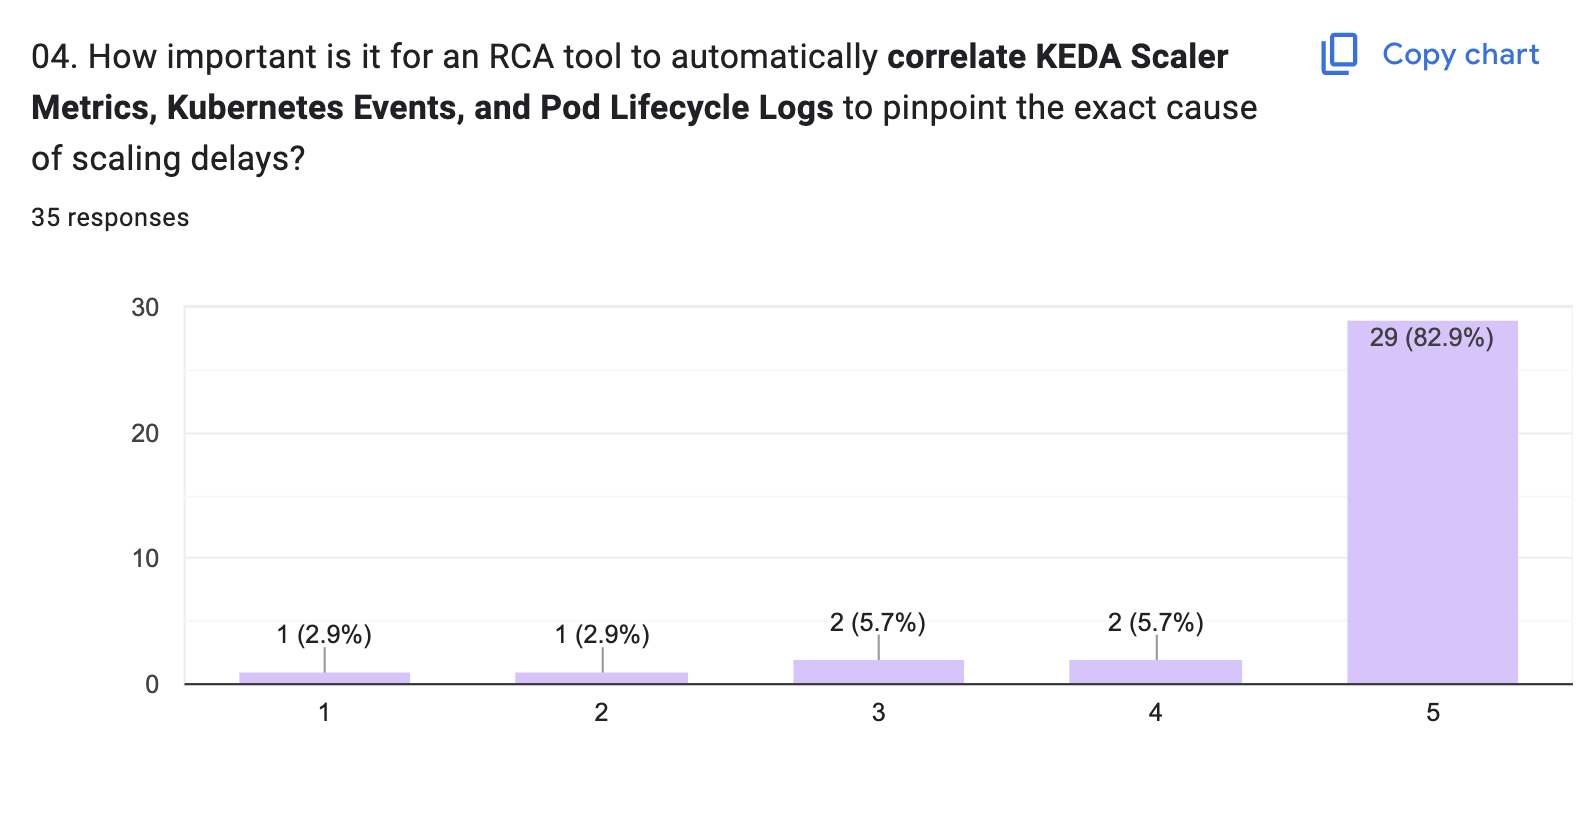
\includegraphics[width=\textwidth]{assets/survey/Q4.png}
\caption{Importance of quantified confidence scores}
\label{fig:app_q4}
\end{figure}

\begin{figure}[H]
\centering
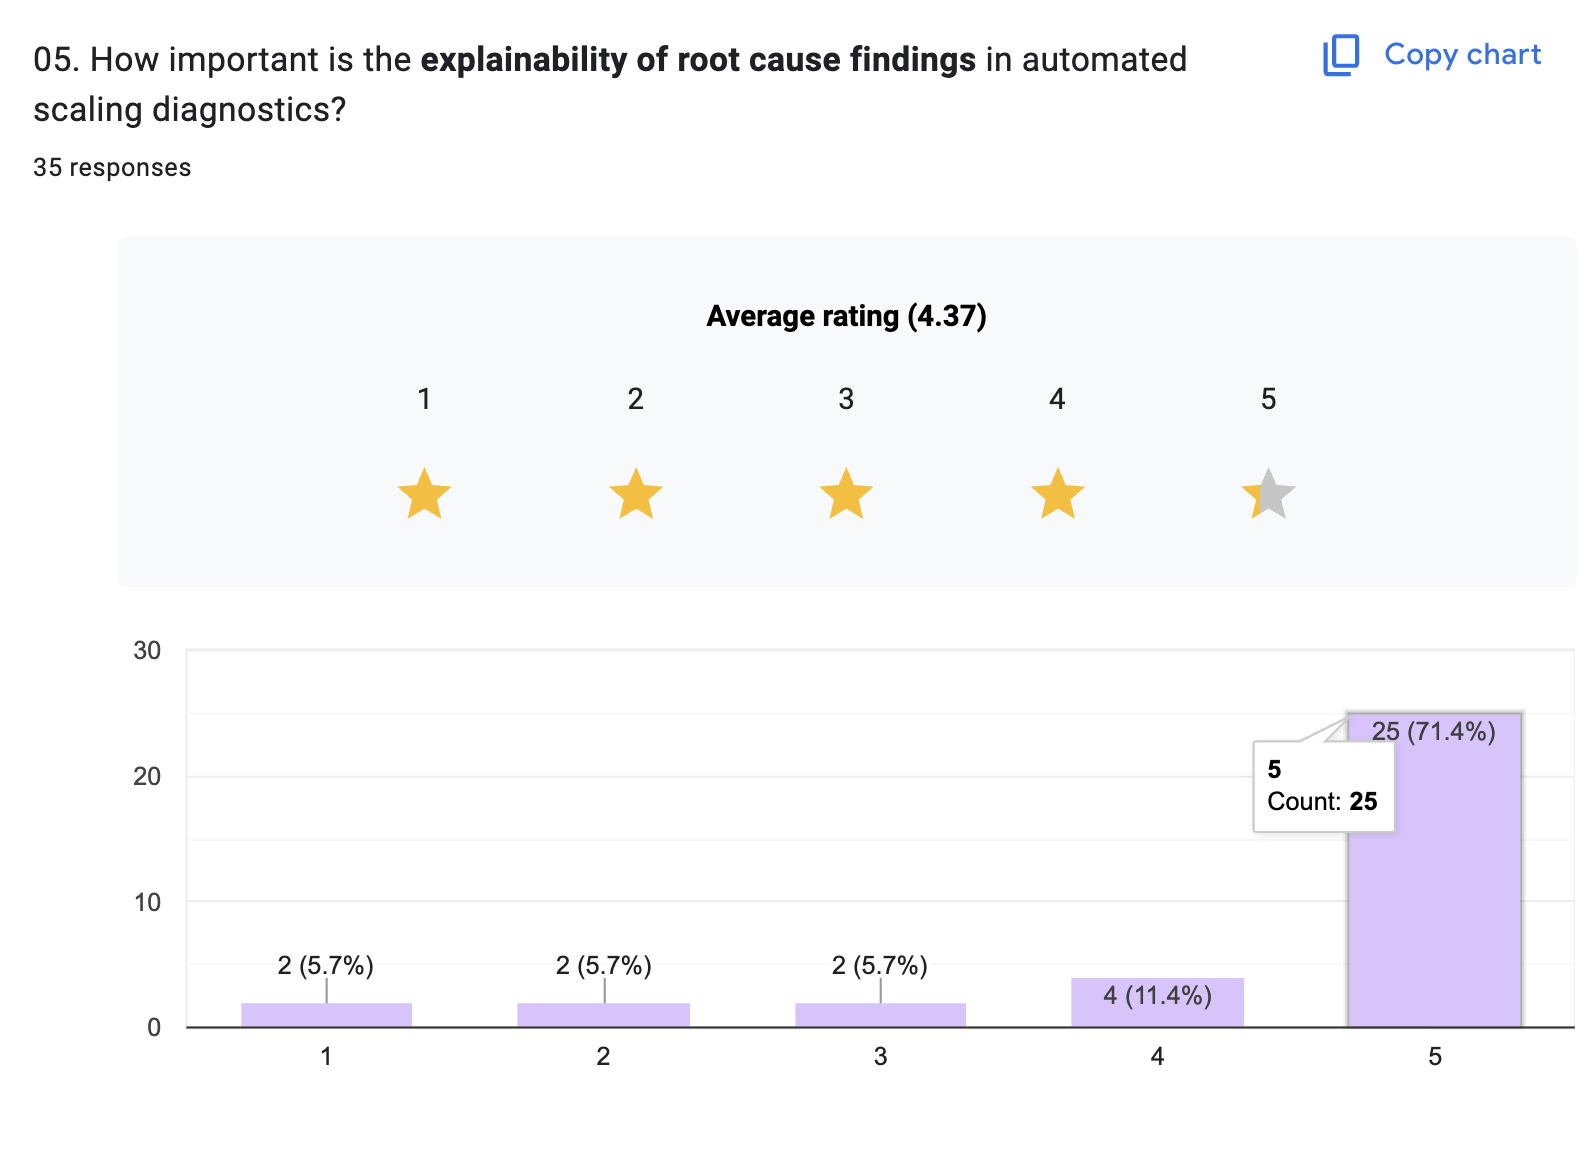
\includegraphics[width=\textwidth]{assets/survey/Q5.png}
\caption{Maximum acceptable RCA latency}
\label{fig:app_q5}
\end{figure}

\begin{figure}[H]
\centering
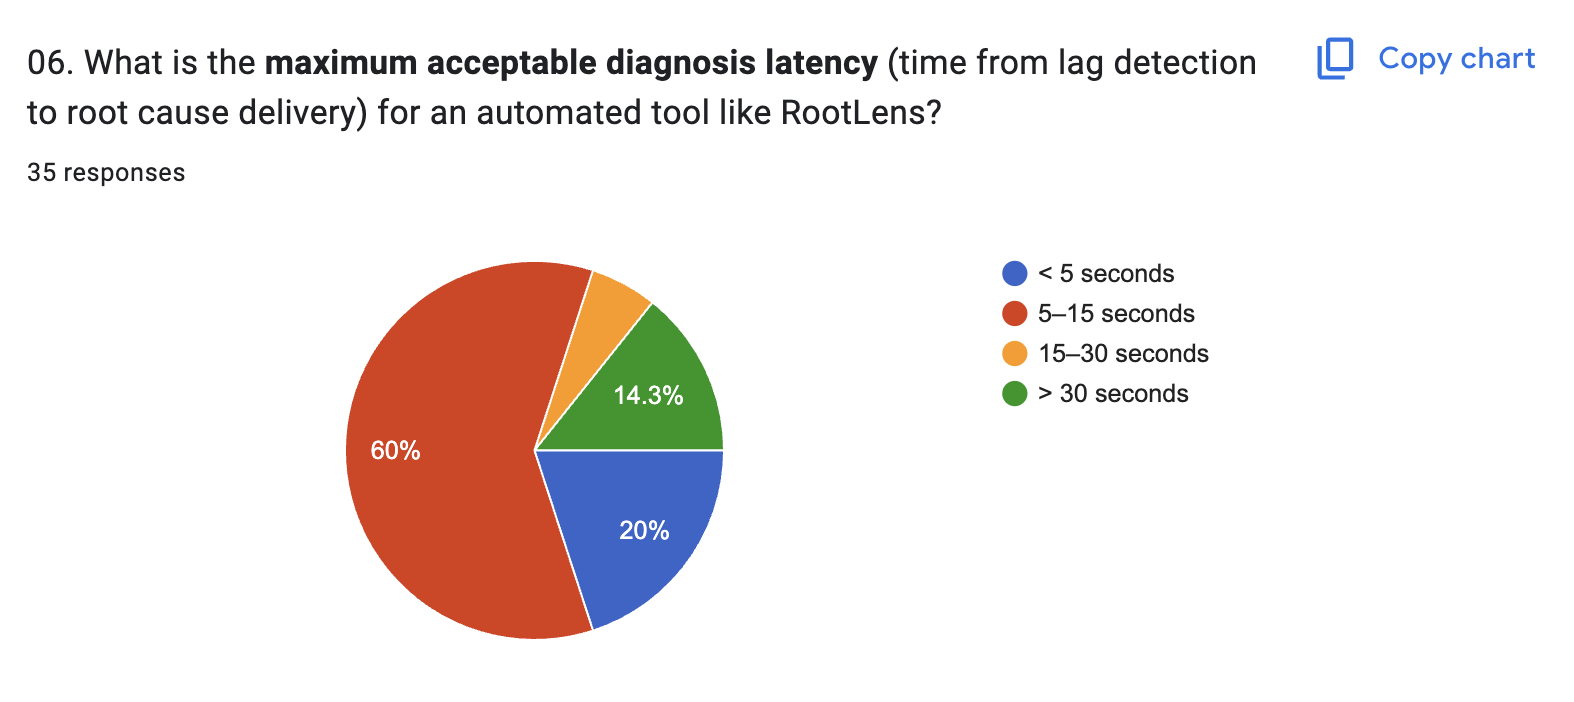
\includegraphics[width=\textwidth]{assets/survey/Q6.png}
\caption{Usefulness of sub-cause granularity}
\label{fig:app_q6}
\end{figure}

\begin{figure}[H]
\centering
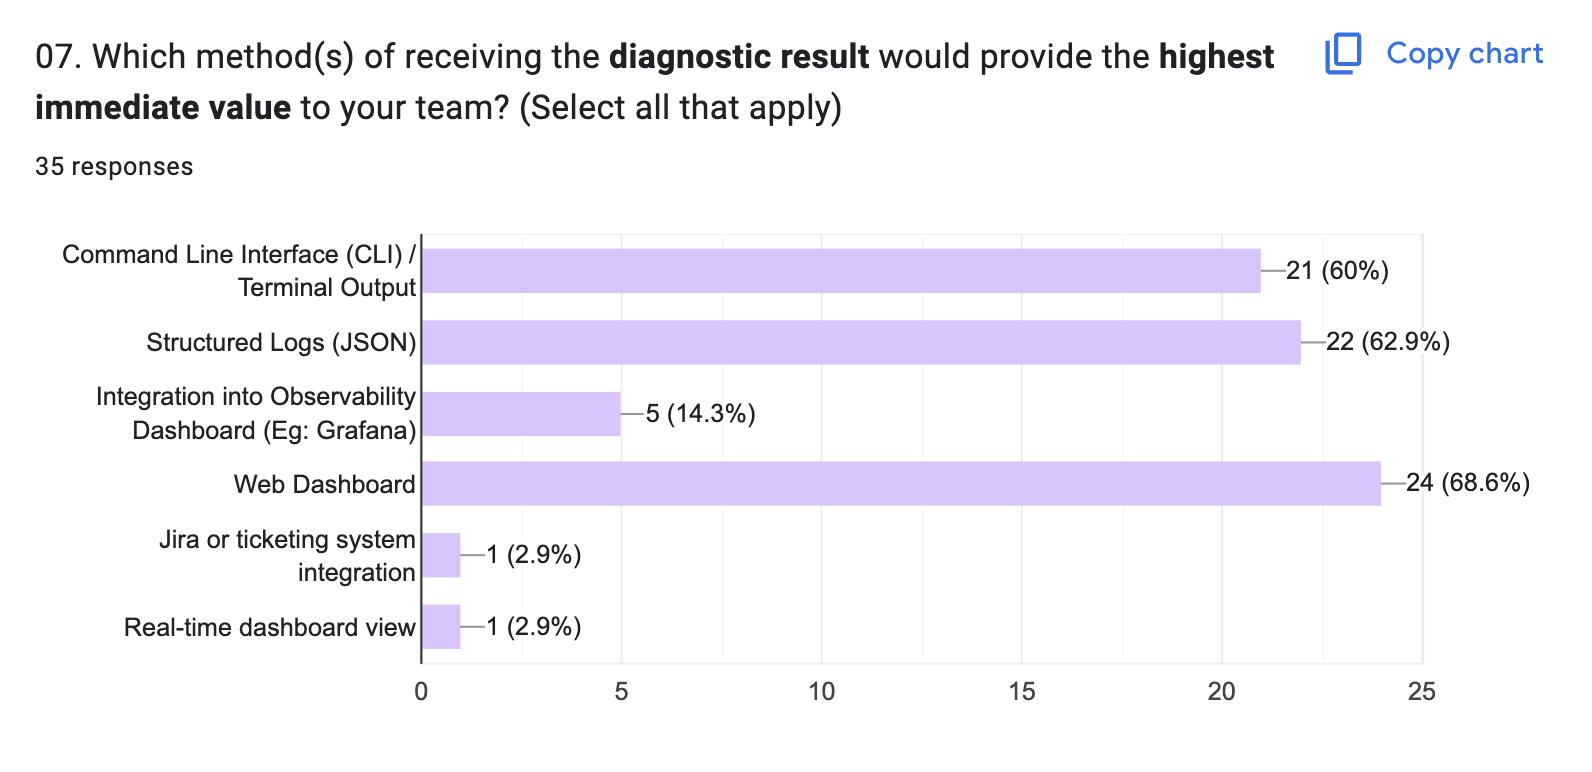
\includegraphics[width=\textwidth]{assets/survey/Q7.png}
\caption{Highest priority dashboard feature}
\label{fig:app_q7}
\end{figure}

\begin{figure}[H]
\centering
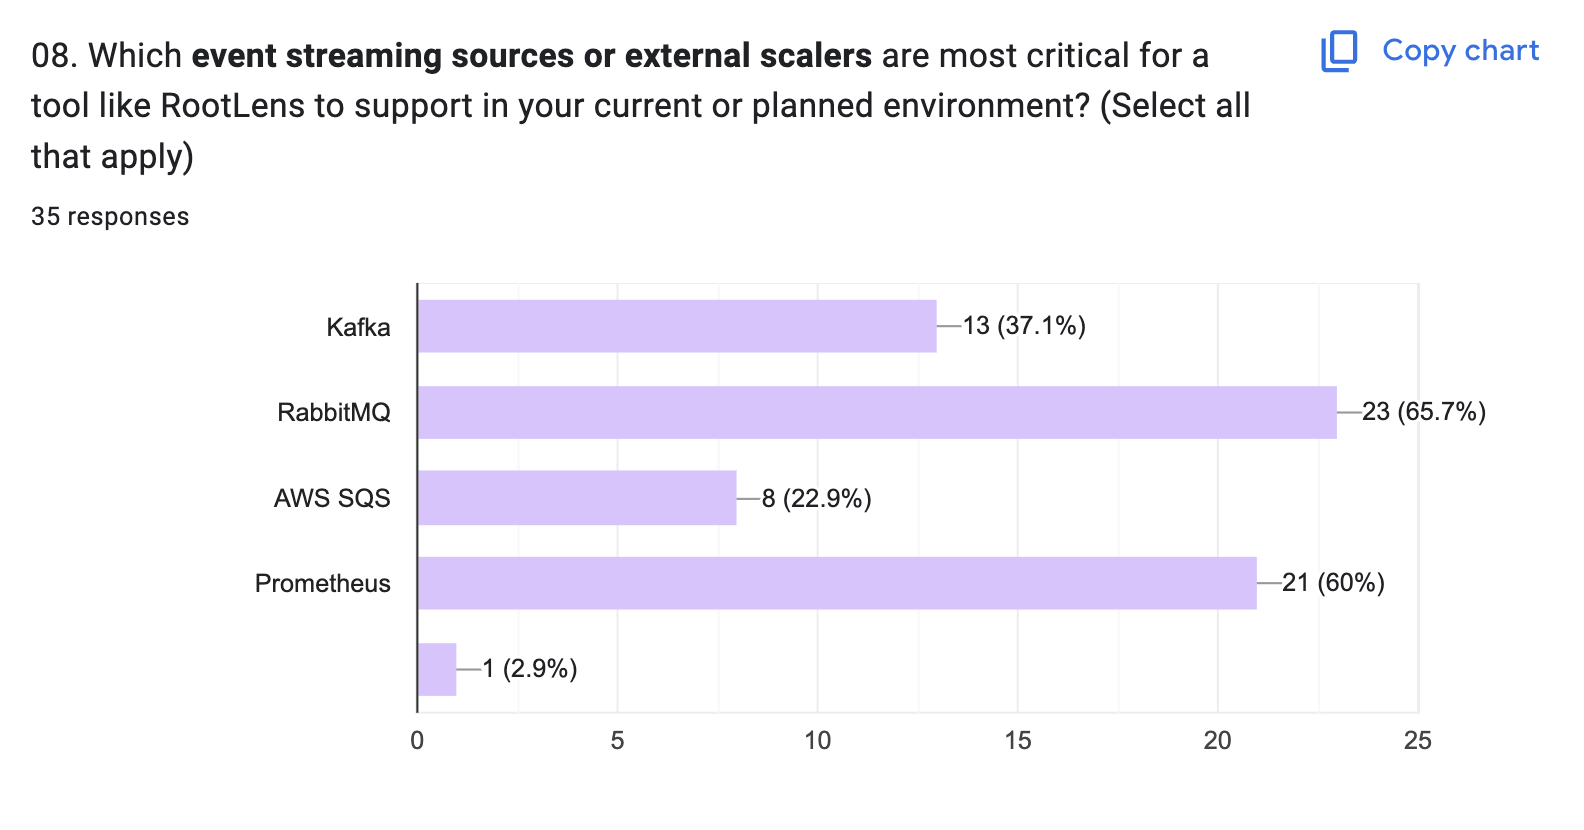
\includegraphics[width=\textwidth]{assets/survey/Q8.png}
\caption{Importance of historical trend view}
\label{fig:app_q8}
\end{figure}

\begin{figure}[H]
\centering
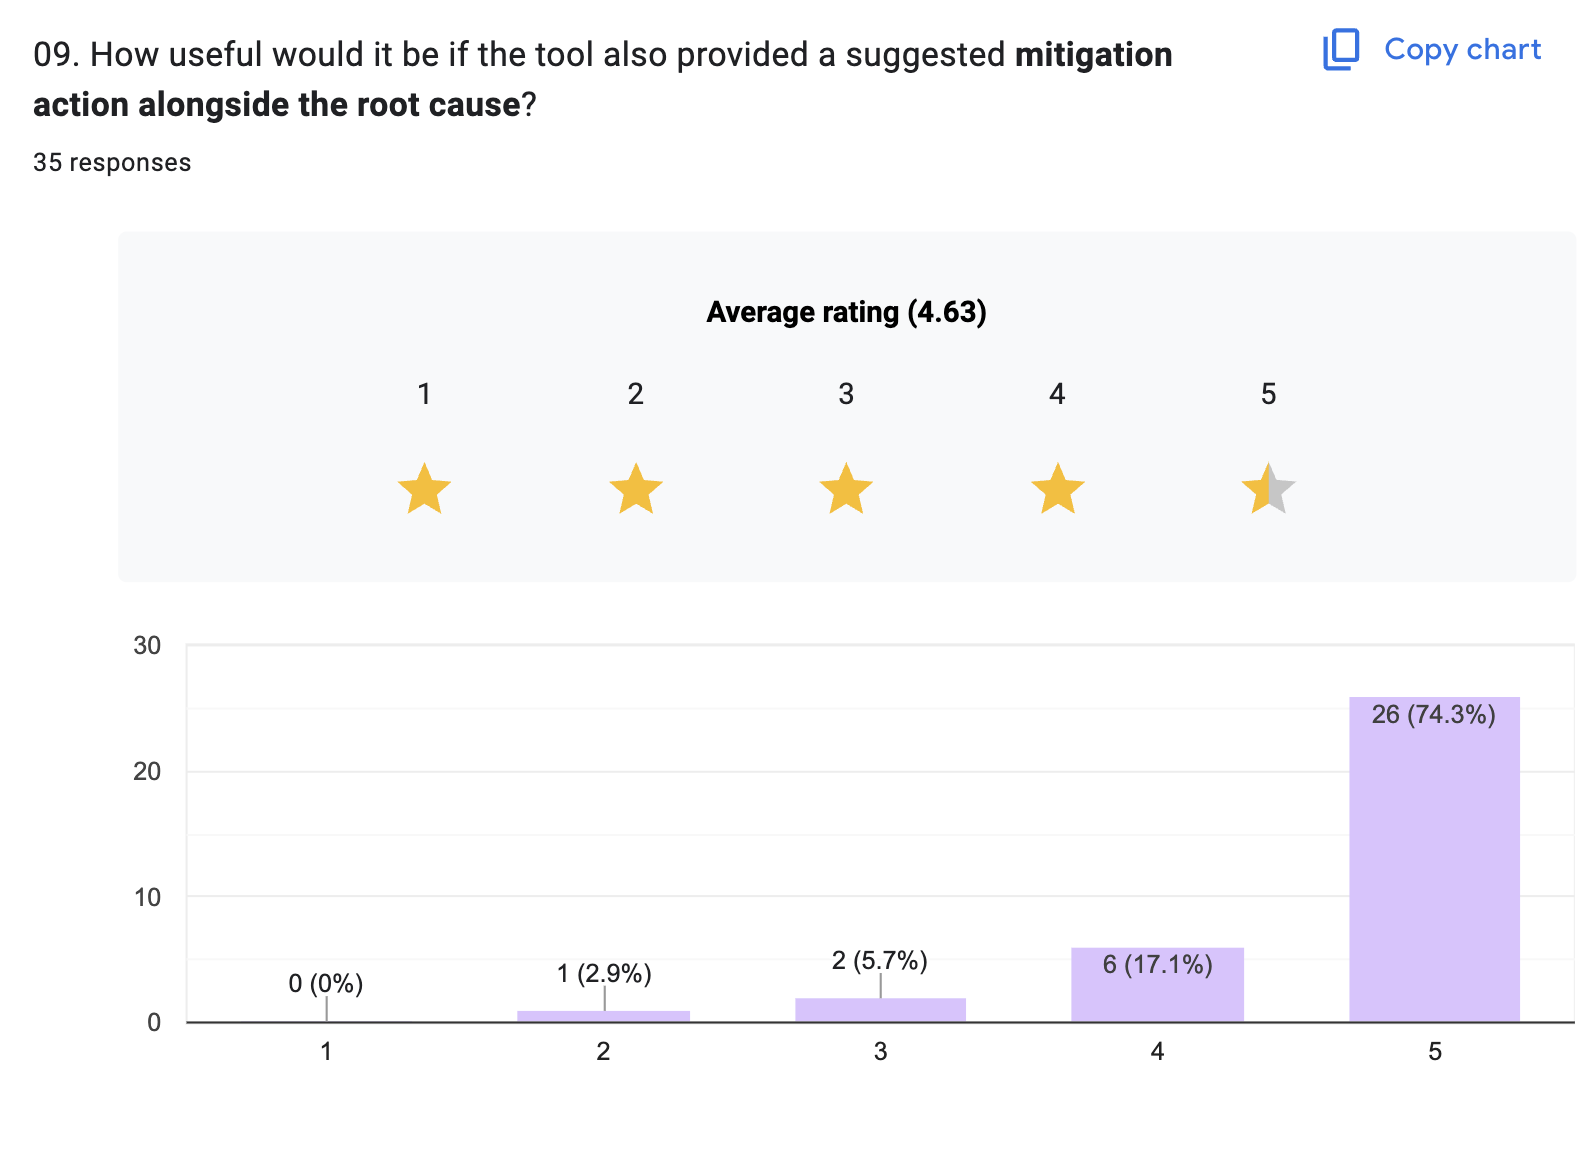
\includegraphics[width=\textwidth]{assets/survey/Q9.png}
\caption{Willingness to integrate automated RCA into alerting}
\label{fig:app_q9}
\end{figure}

\begin{figure}[H]
\centering
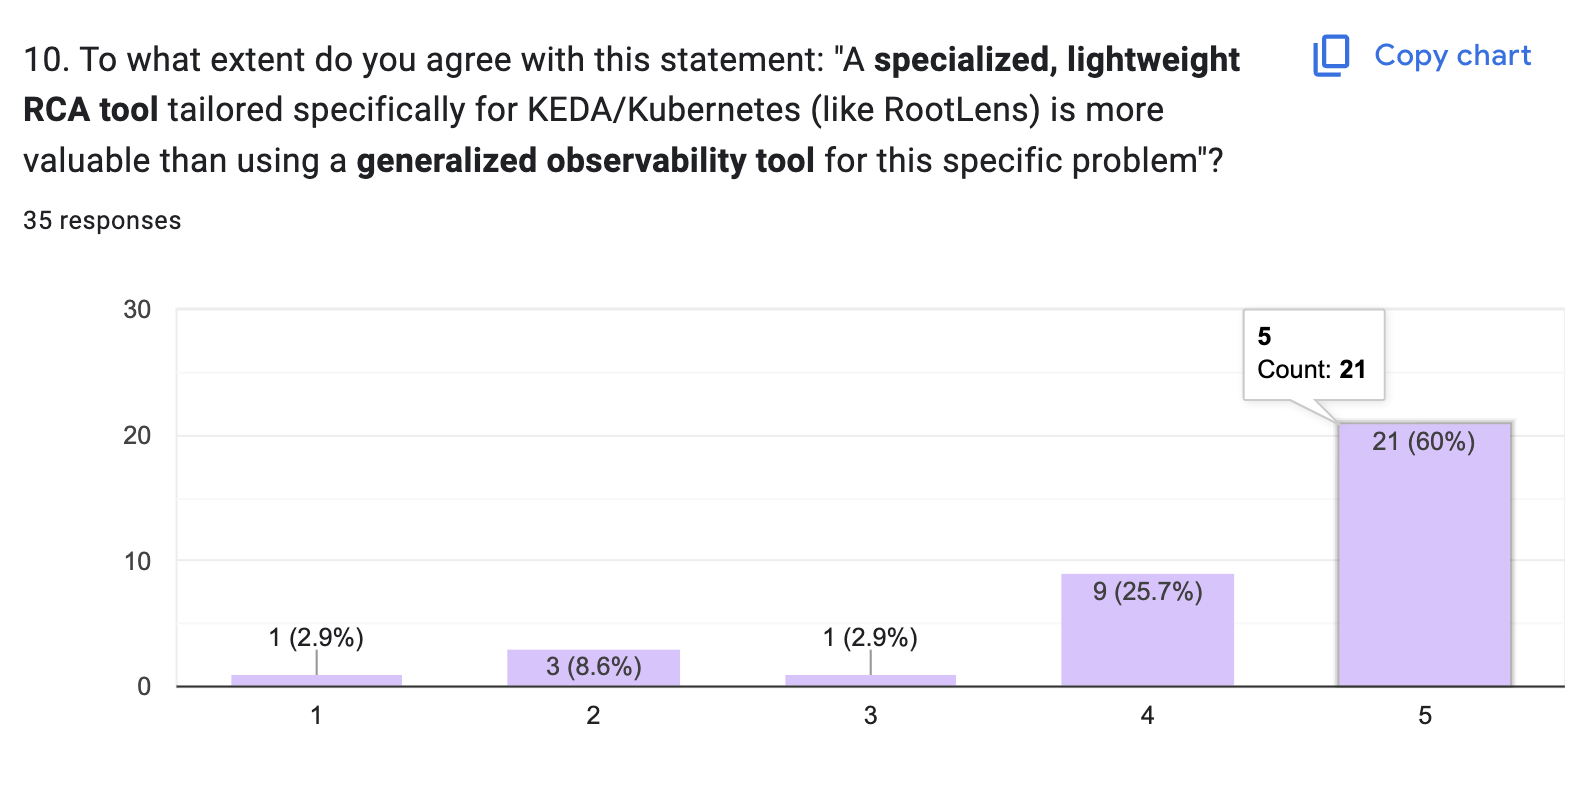
\includegraphics[width=\textwidth]{assets/survey/Q10.png}
\caption{Required confidence threshold for trusting automated diagnosis}
\label{fig:app_q10}
\end{figure}

% ==========================

\section*{Appendix B: Testing Materials}
\addcontentsline{toc}{section}{Appendix B: Testing Materials}

The following listing shows a minikube setup used for the local development.

\begin{figure}[H]
\centering
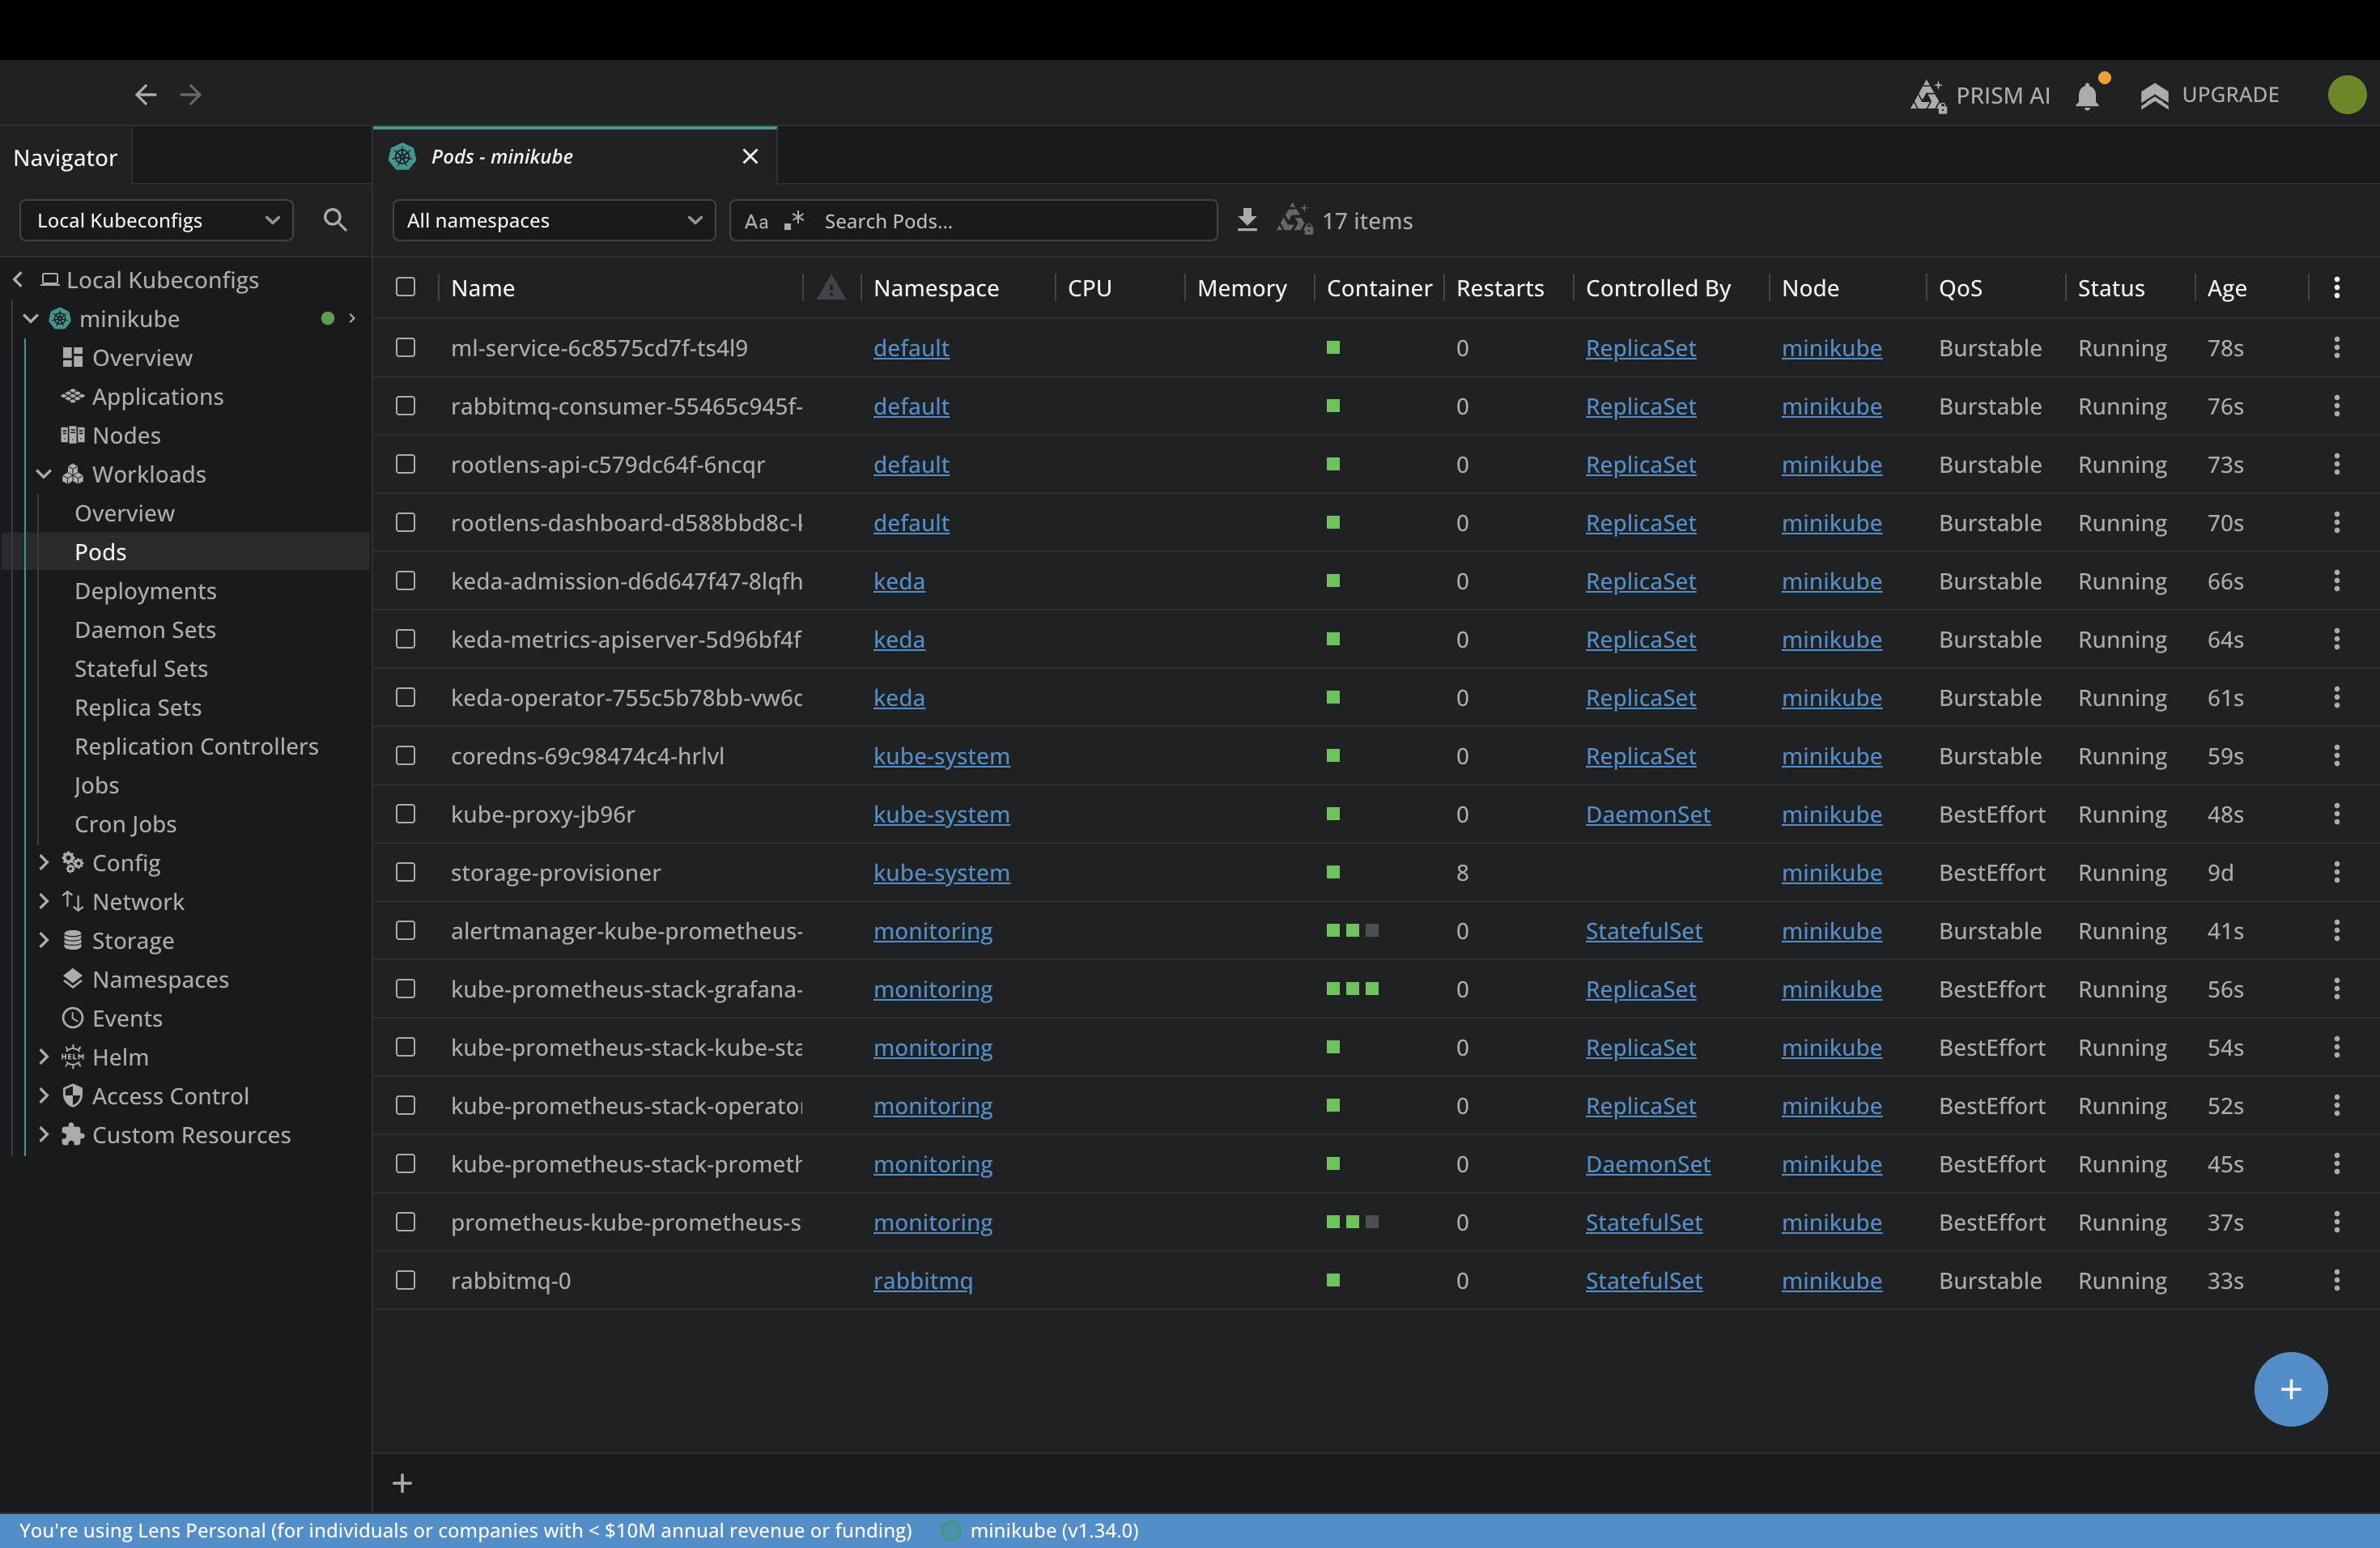
\includegraphics[width=\textwidth]{thesis/assets/minikube_setup.png}
\caption{Minikube Cluster Setup}
\label{fig:minikube}
\end{figure}

% ==========================

\section*{Appendix C: Code Snippets}
\addcontentsline{toc}{section}{Appendix C: Code Snippets}

\begin{figure}[H]
\centering
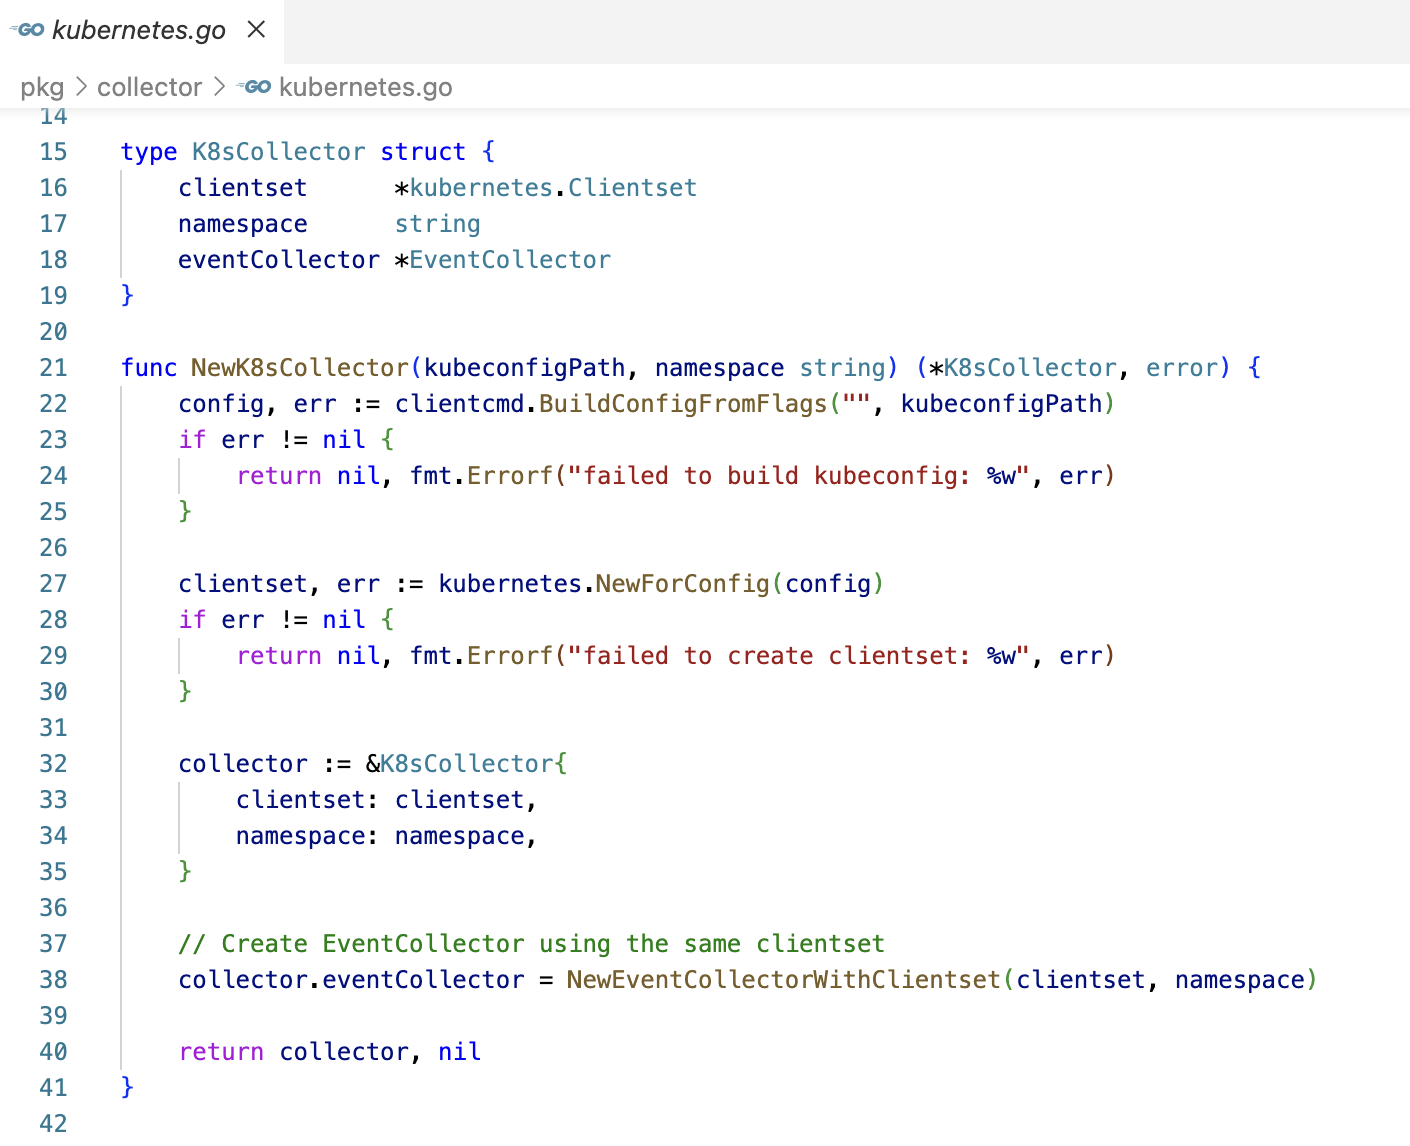
\includegraphics[width=\textwidth, height=0.4\textheight, keepaspectratio]{thesis/assets/kubernetes_collector.png}
\caption{Code - Kubernetes Collector}
\label{fig:collector_1}
\end{figure}

\begin{figure}[H]
\centering
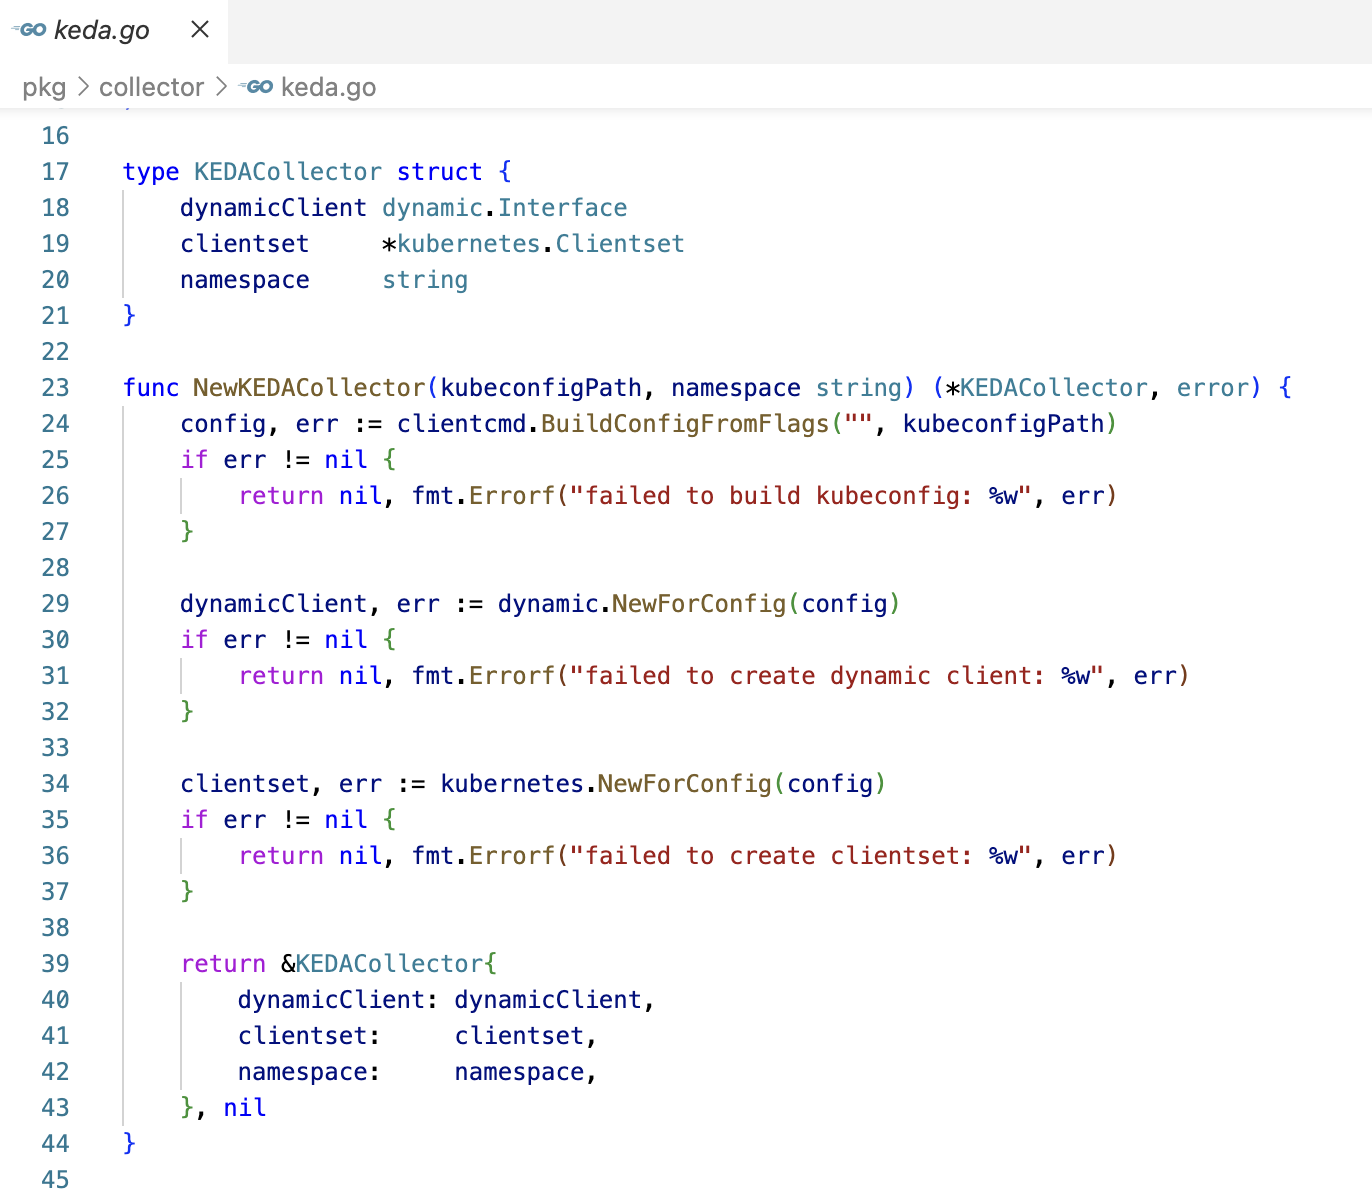
\includegraphics[width=\textwidth, height=0.4\textheight, keepaspectratio]{thesis/assets/keda_collector.png}
\caption{Code - Keda Collector}
\label{fig:collector_2}
\end{figure}

\begin{figure}[H]
\centering
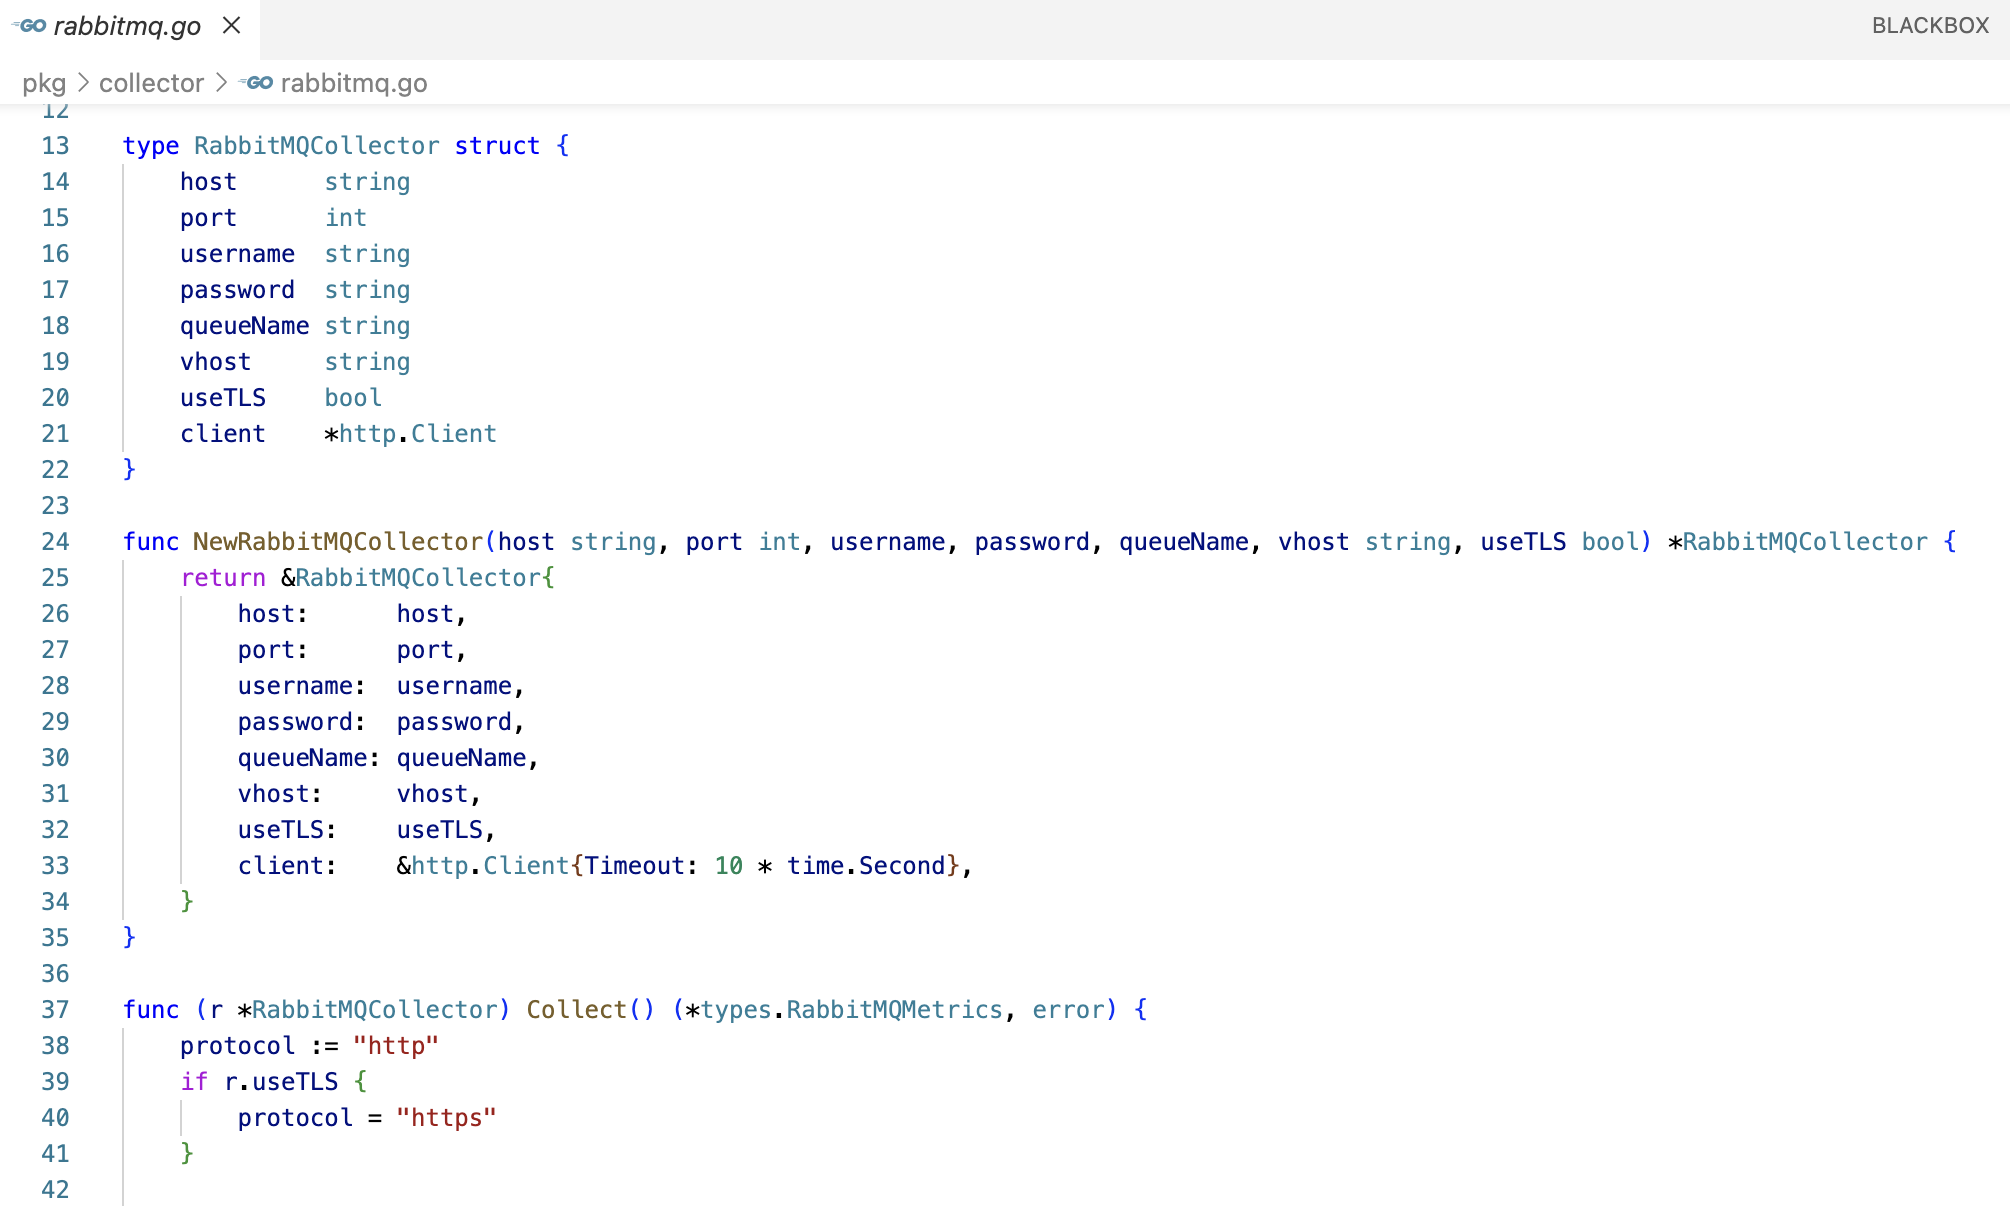
\includegraphics[width=\textwidth, height=0.4\textheight, keepaspectratio]{thesis/assets/rabbitmq_collector.png}
\caption{Code - Rabbitmq Collector}
\label{fig:collector_3}
\end{figure}

\begin{figure}[H]
\centering
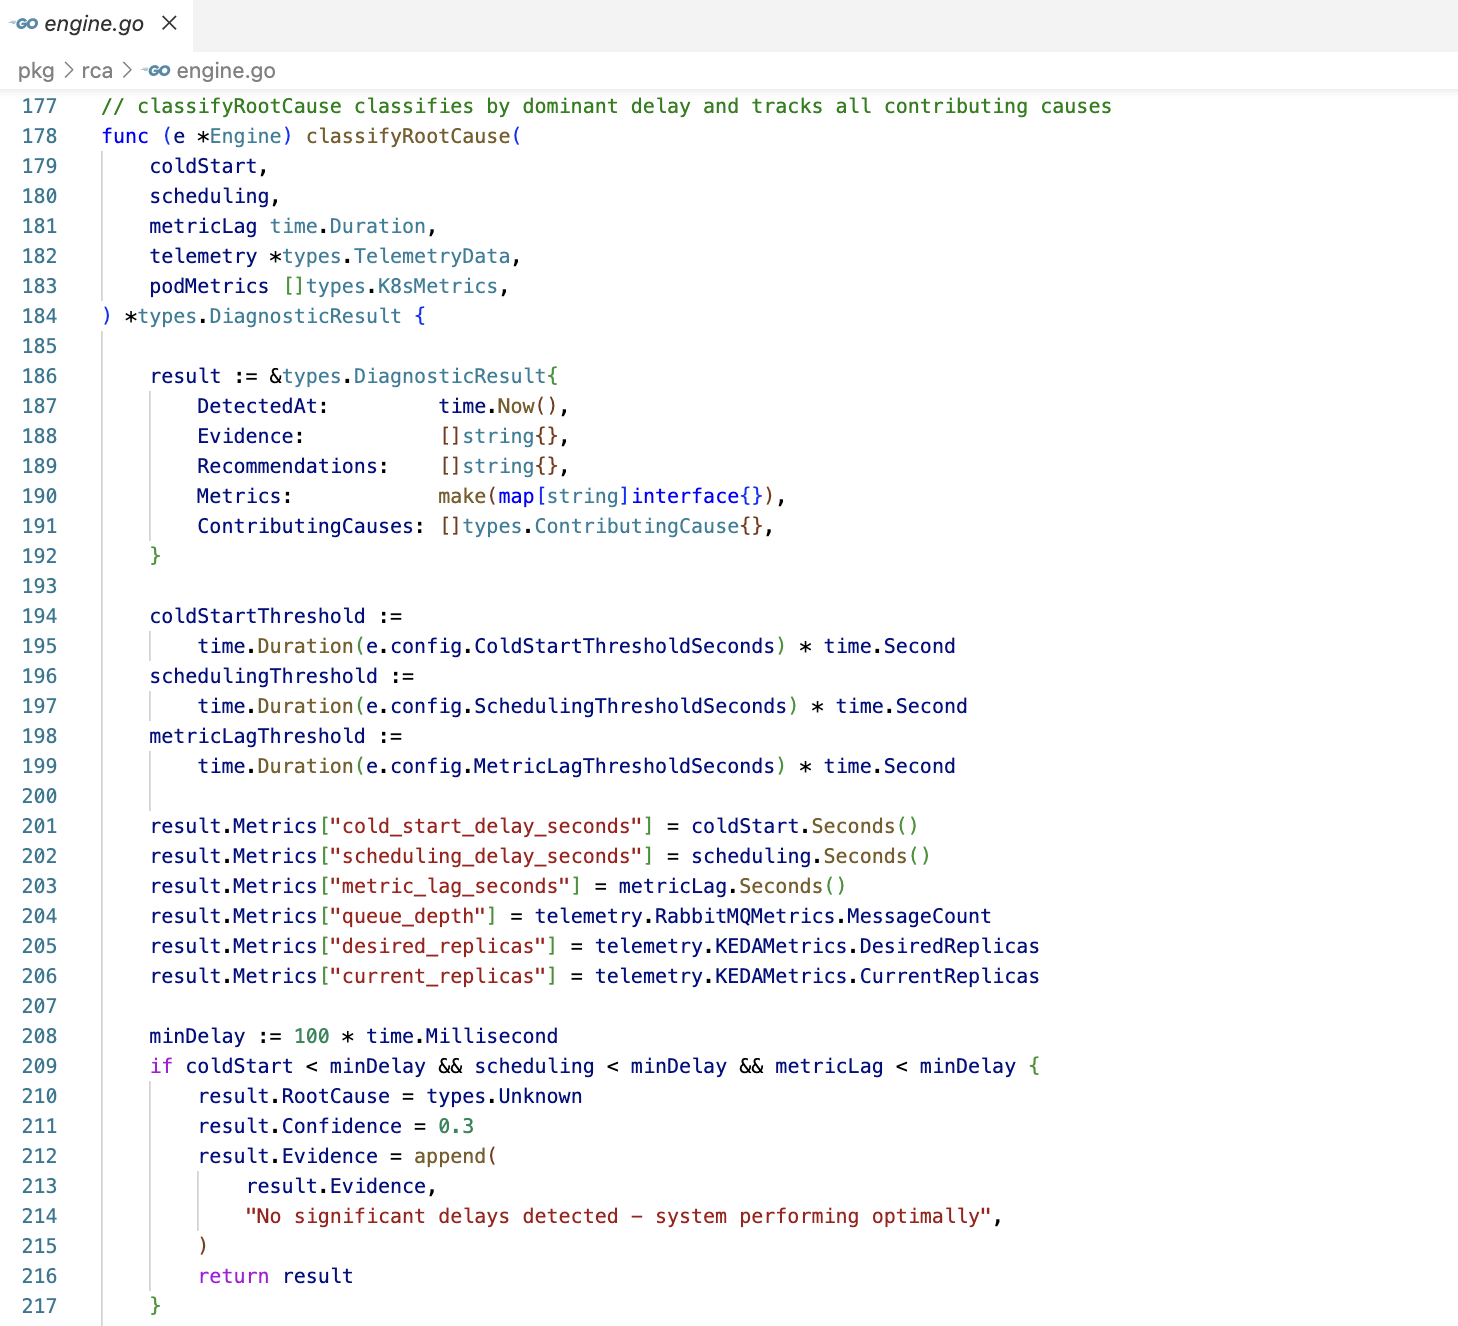
\includegraphics[width=\textwidth, height=0.4\textheight, keepaspectratio]{thesis/assets/rca_logic.png}
\caption{Code - RCA Logic}
\label{fig:rca_logic}
\end{figure}

\begin{figure}[H]
\centering
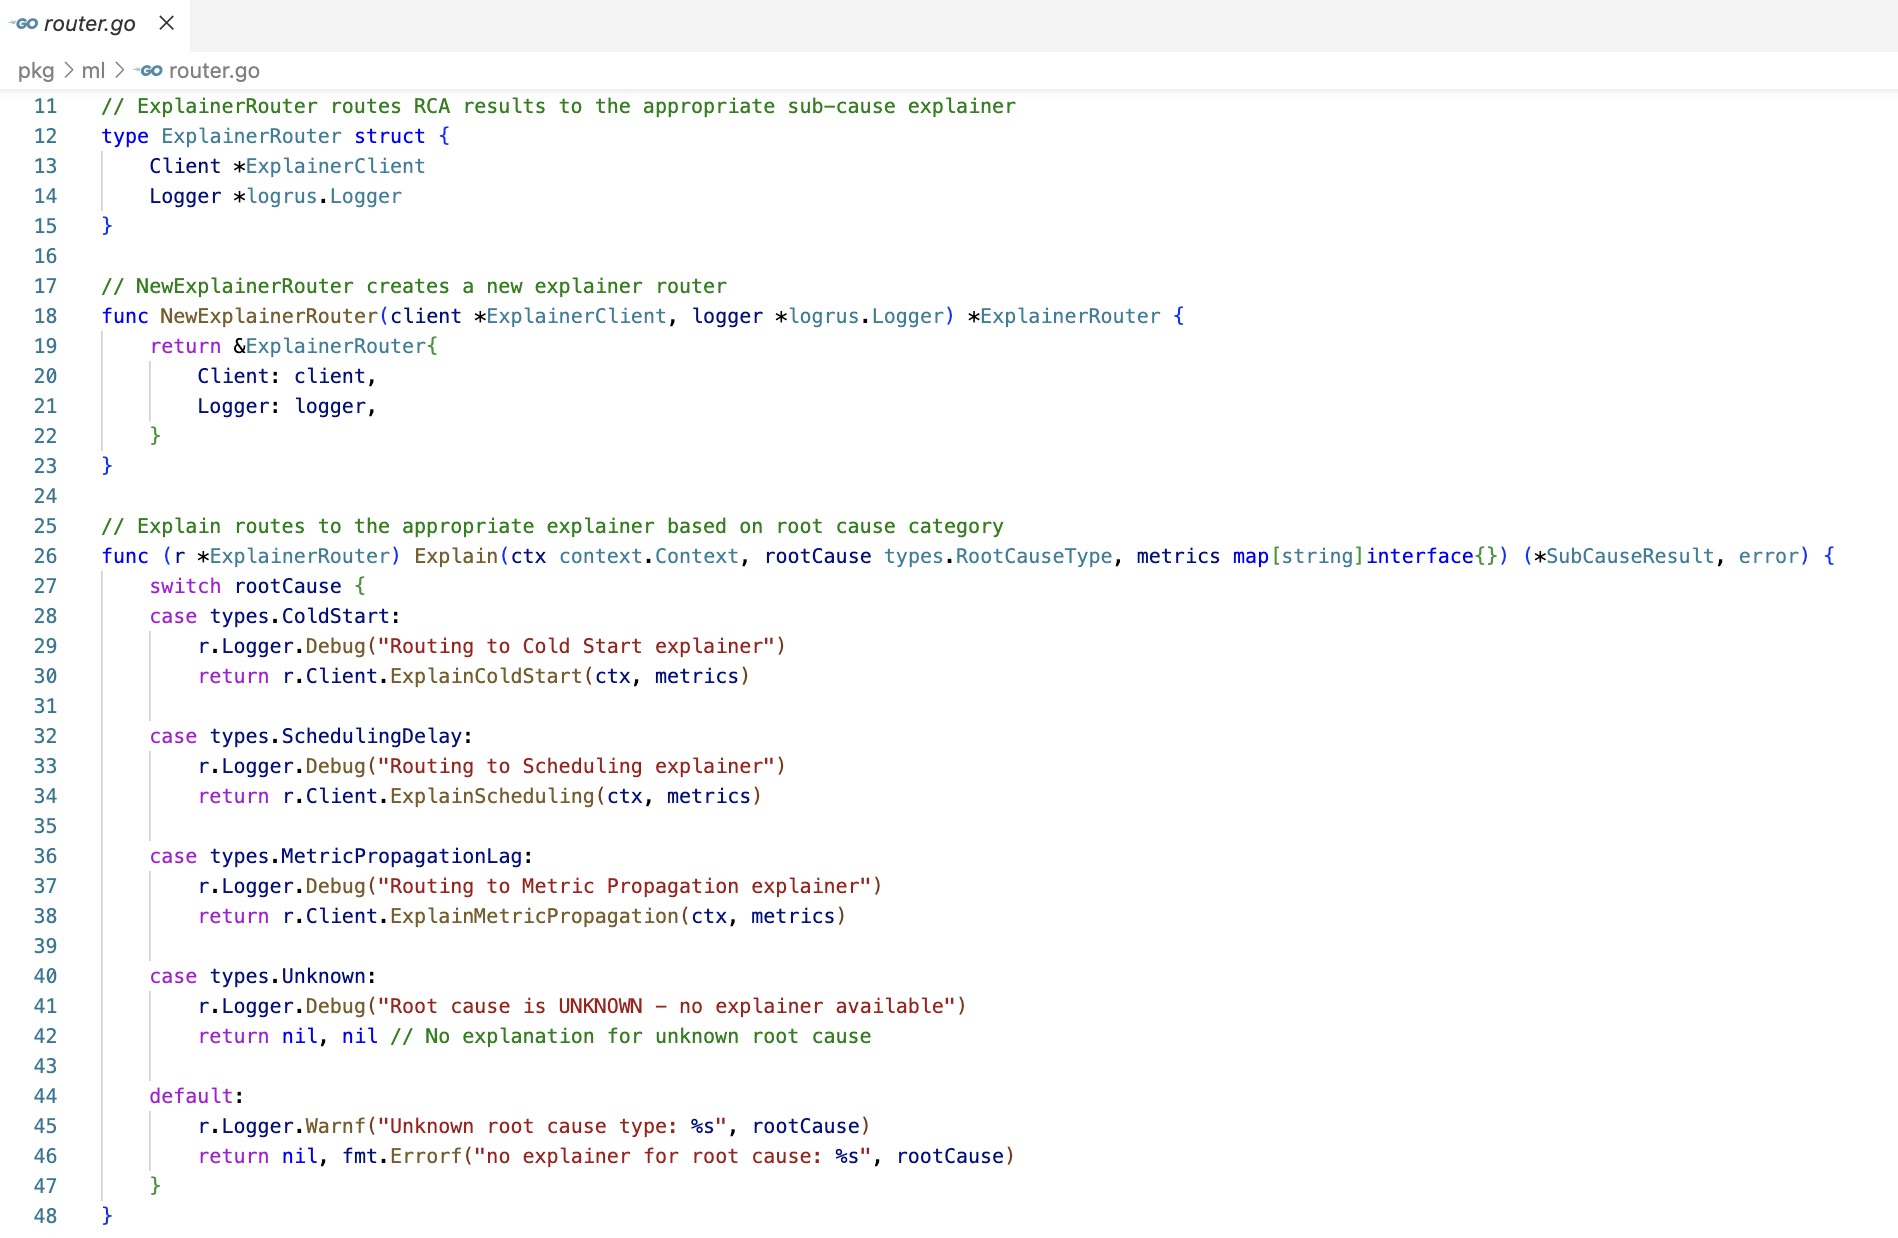
\includegraphics[width=\textwidth, height=0.4\textheight, keepaspectratio]{thesis/assets/explainer_router.png}
\caption{Code - ML Explainer Router}
\label{fig:ml_explainer}
\end{figure}

% ==========================

\section*{Appendix D: System UI/UX}
\addcontentsline{toc}{section}{Appendix D: System UI/UX}

\begin{figure}[H]
\centering
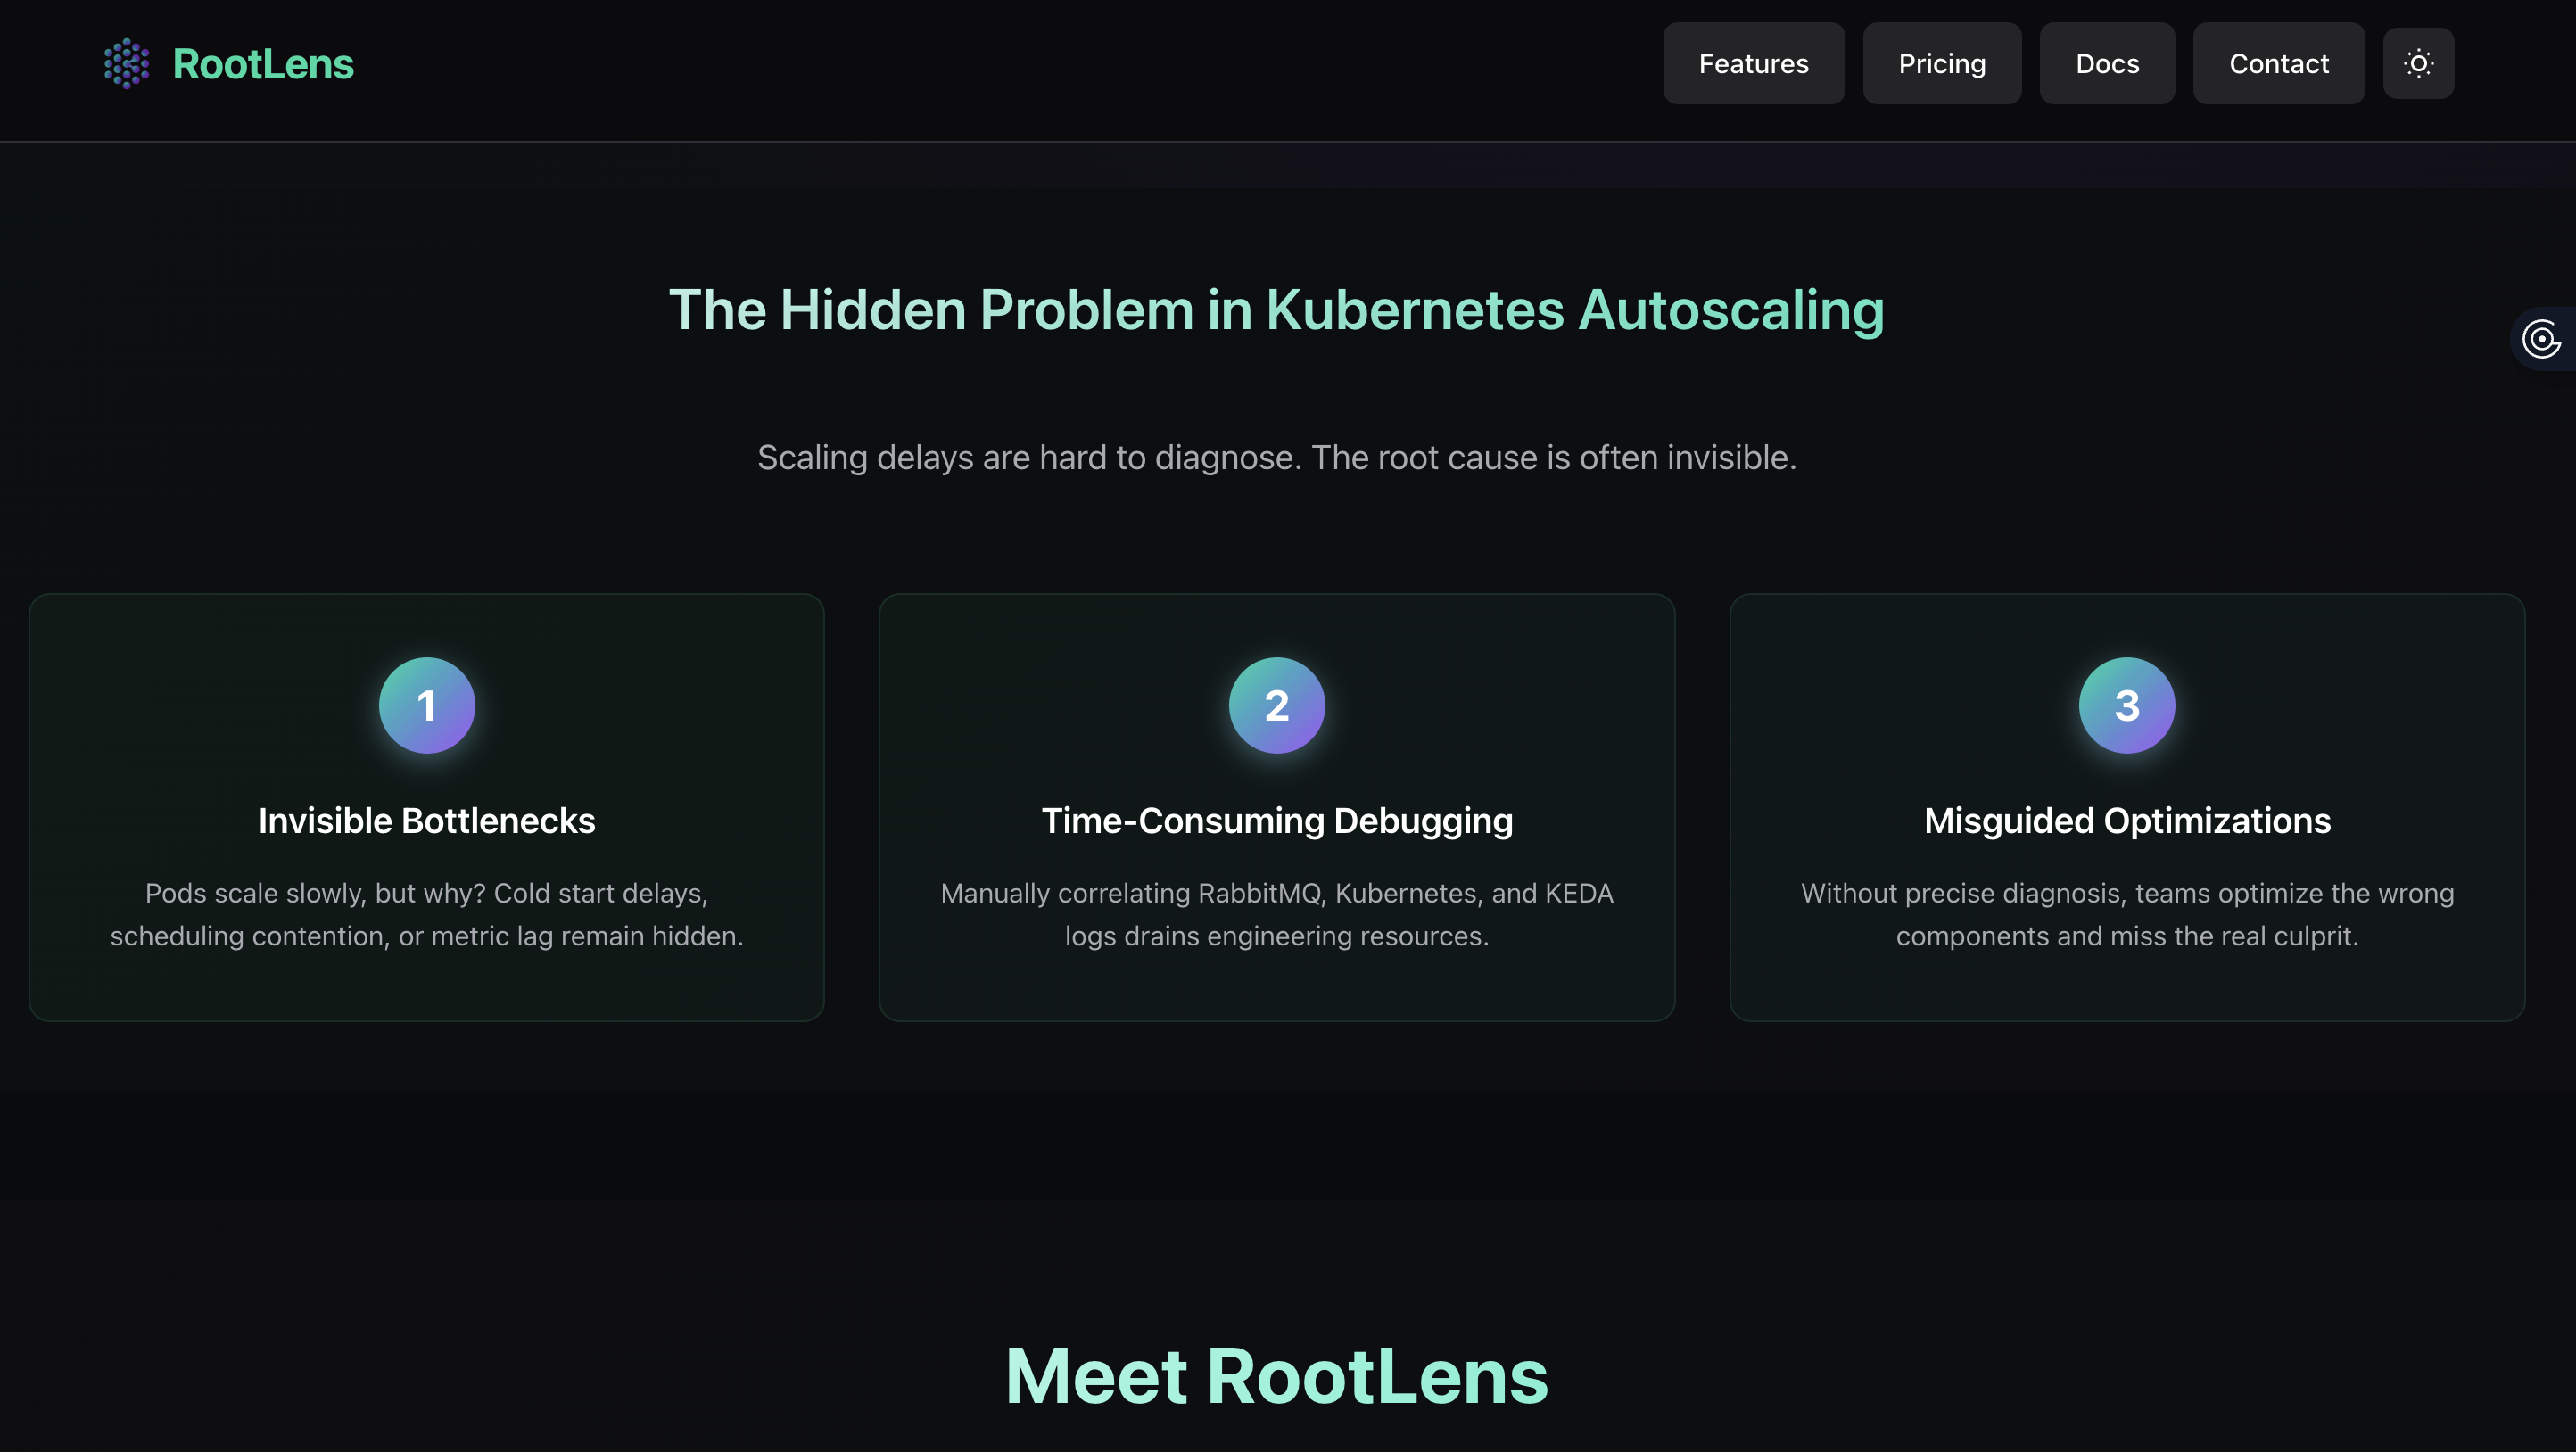
\includegraphics[width=\textwidth]{thesis/assets/main-2.png}
\caption{Marketing Website Page 2}
\label{fig:app_main2}
\end{figure}

\begin{figure}[H]
\centering
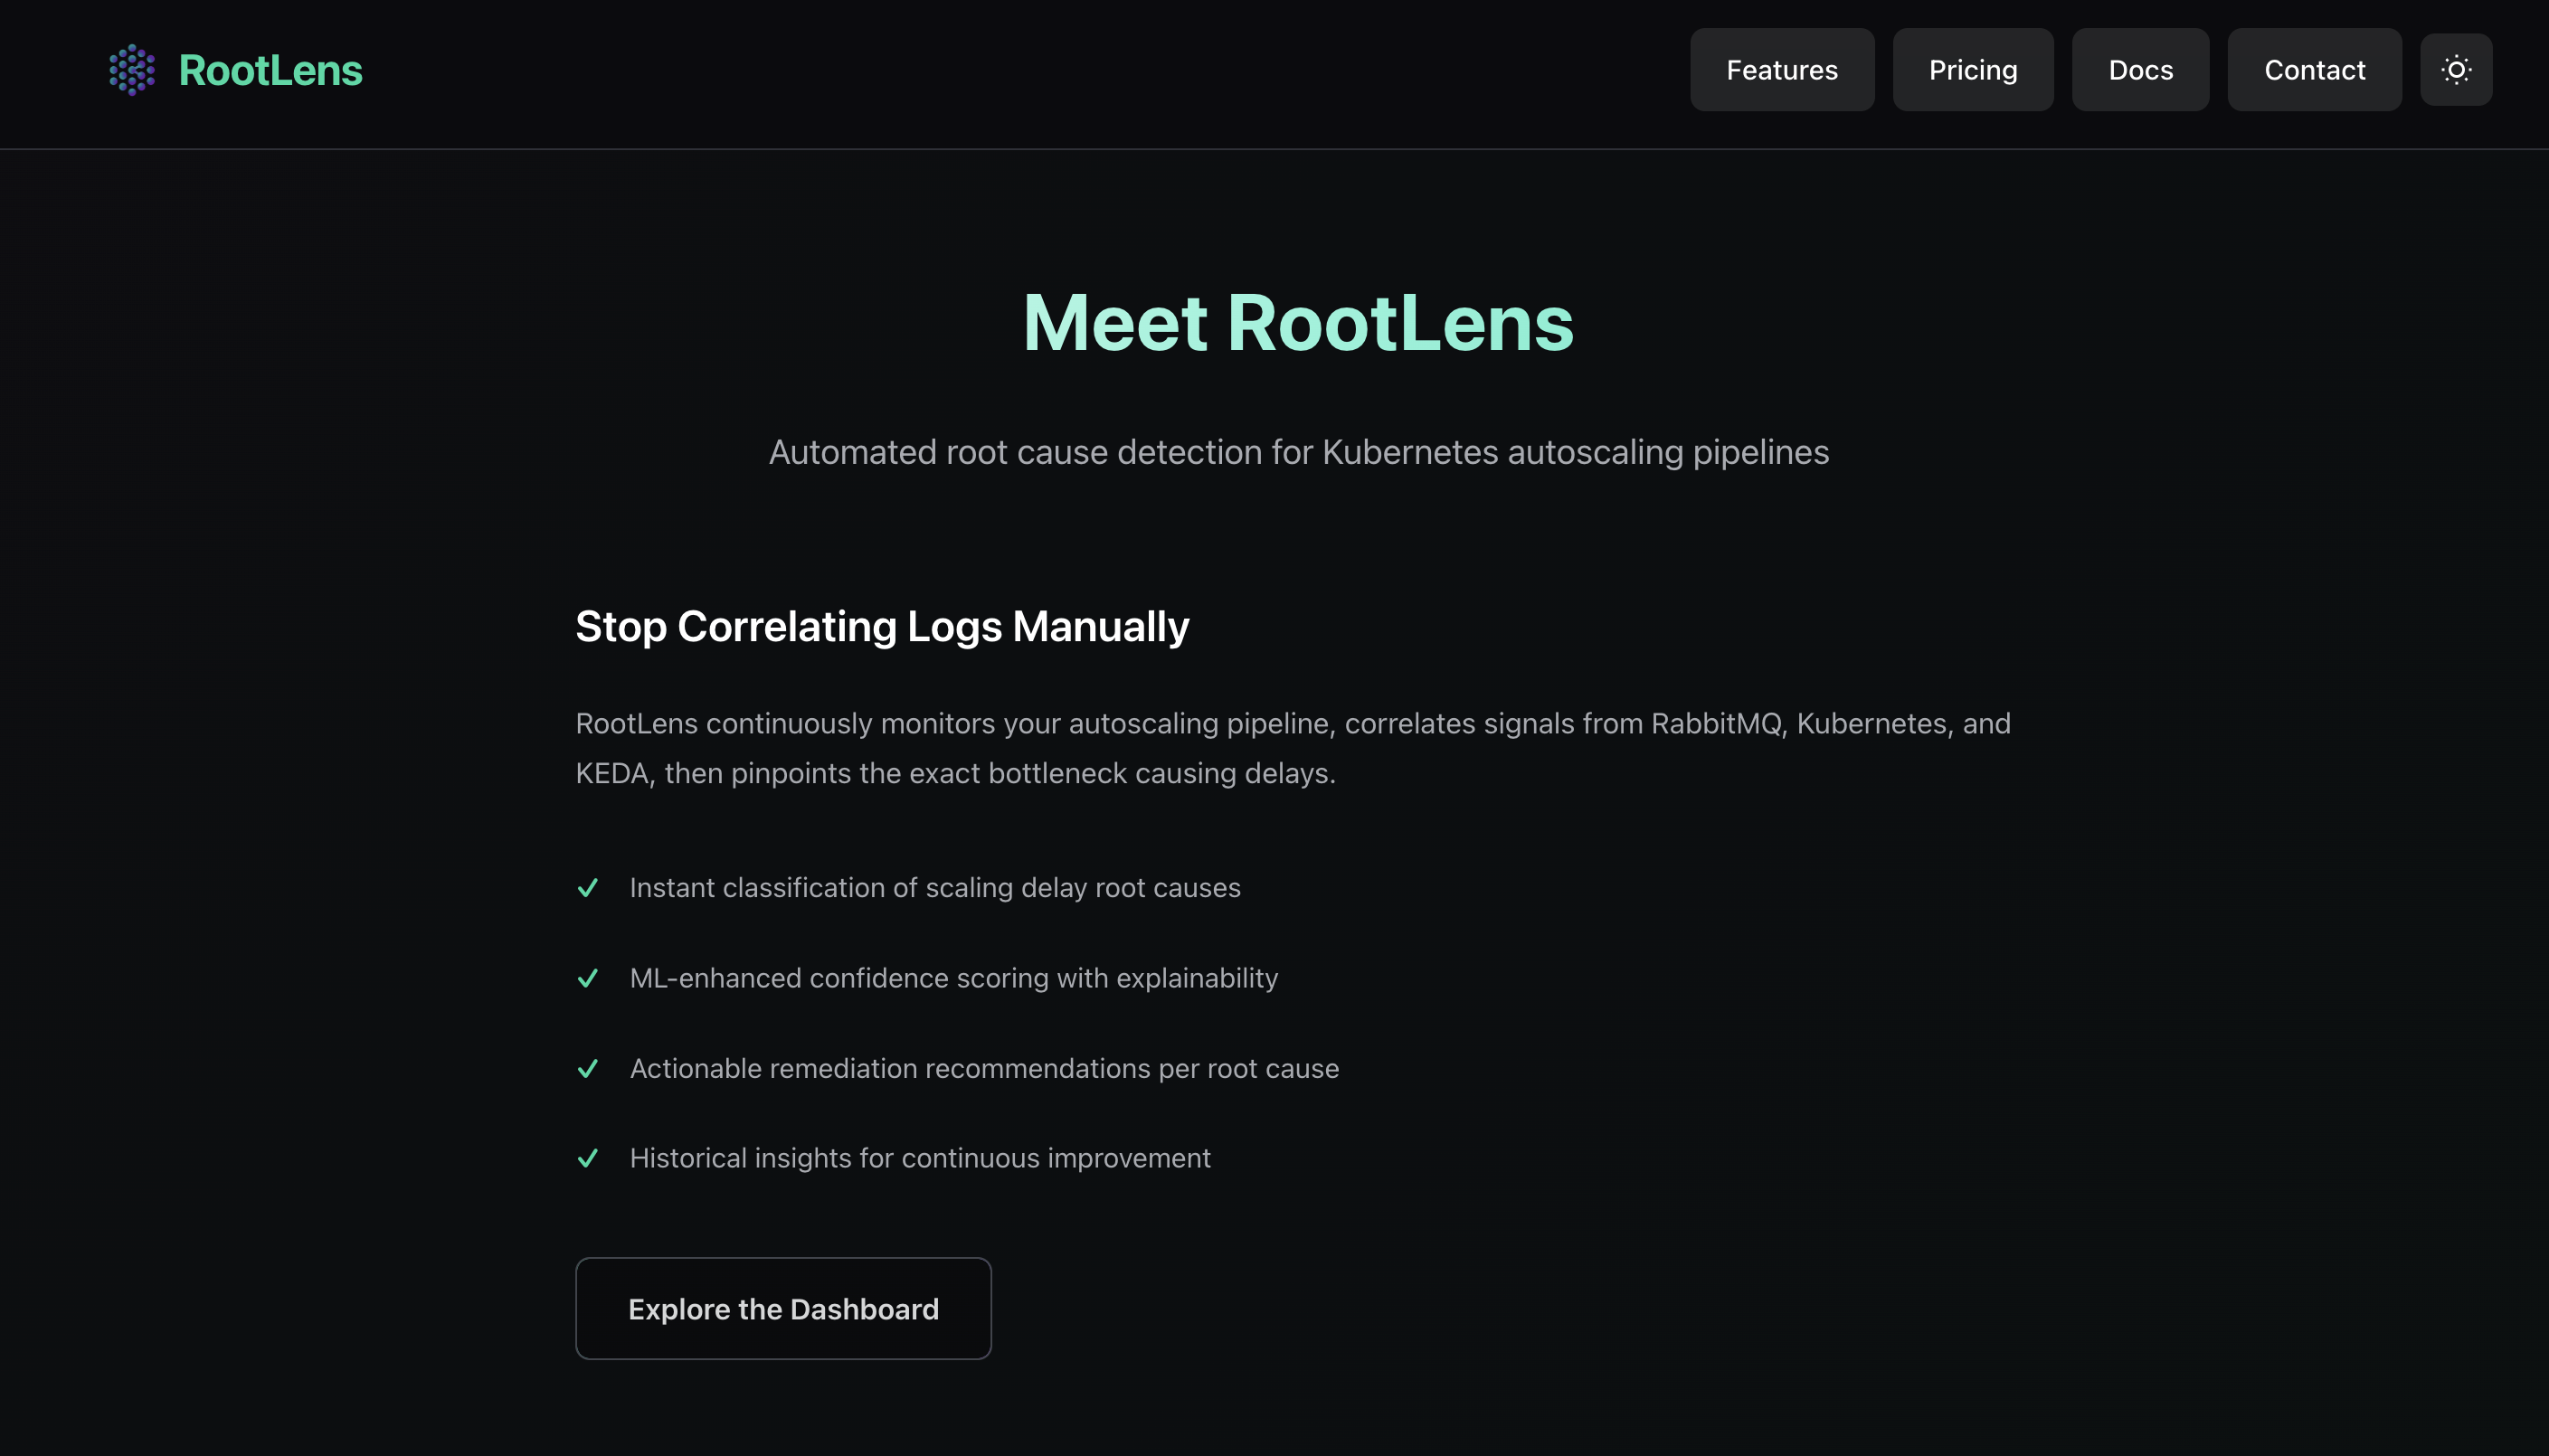
\includegraphics[width=\textwidth]{thesis/assets/main-3.png}
\caption{Marketing Website Page 3}
\label{fig:app_main3}
\end{figure}

\begin{figure}[H]
\centering
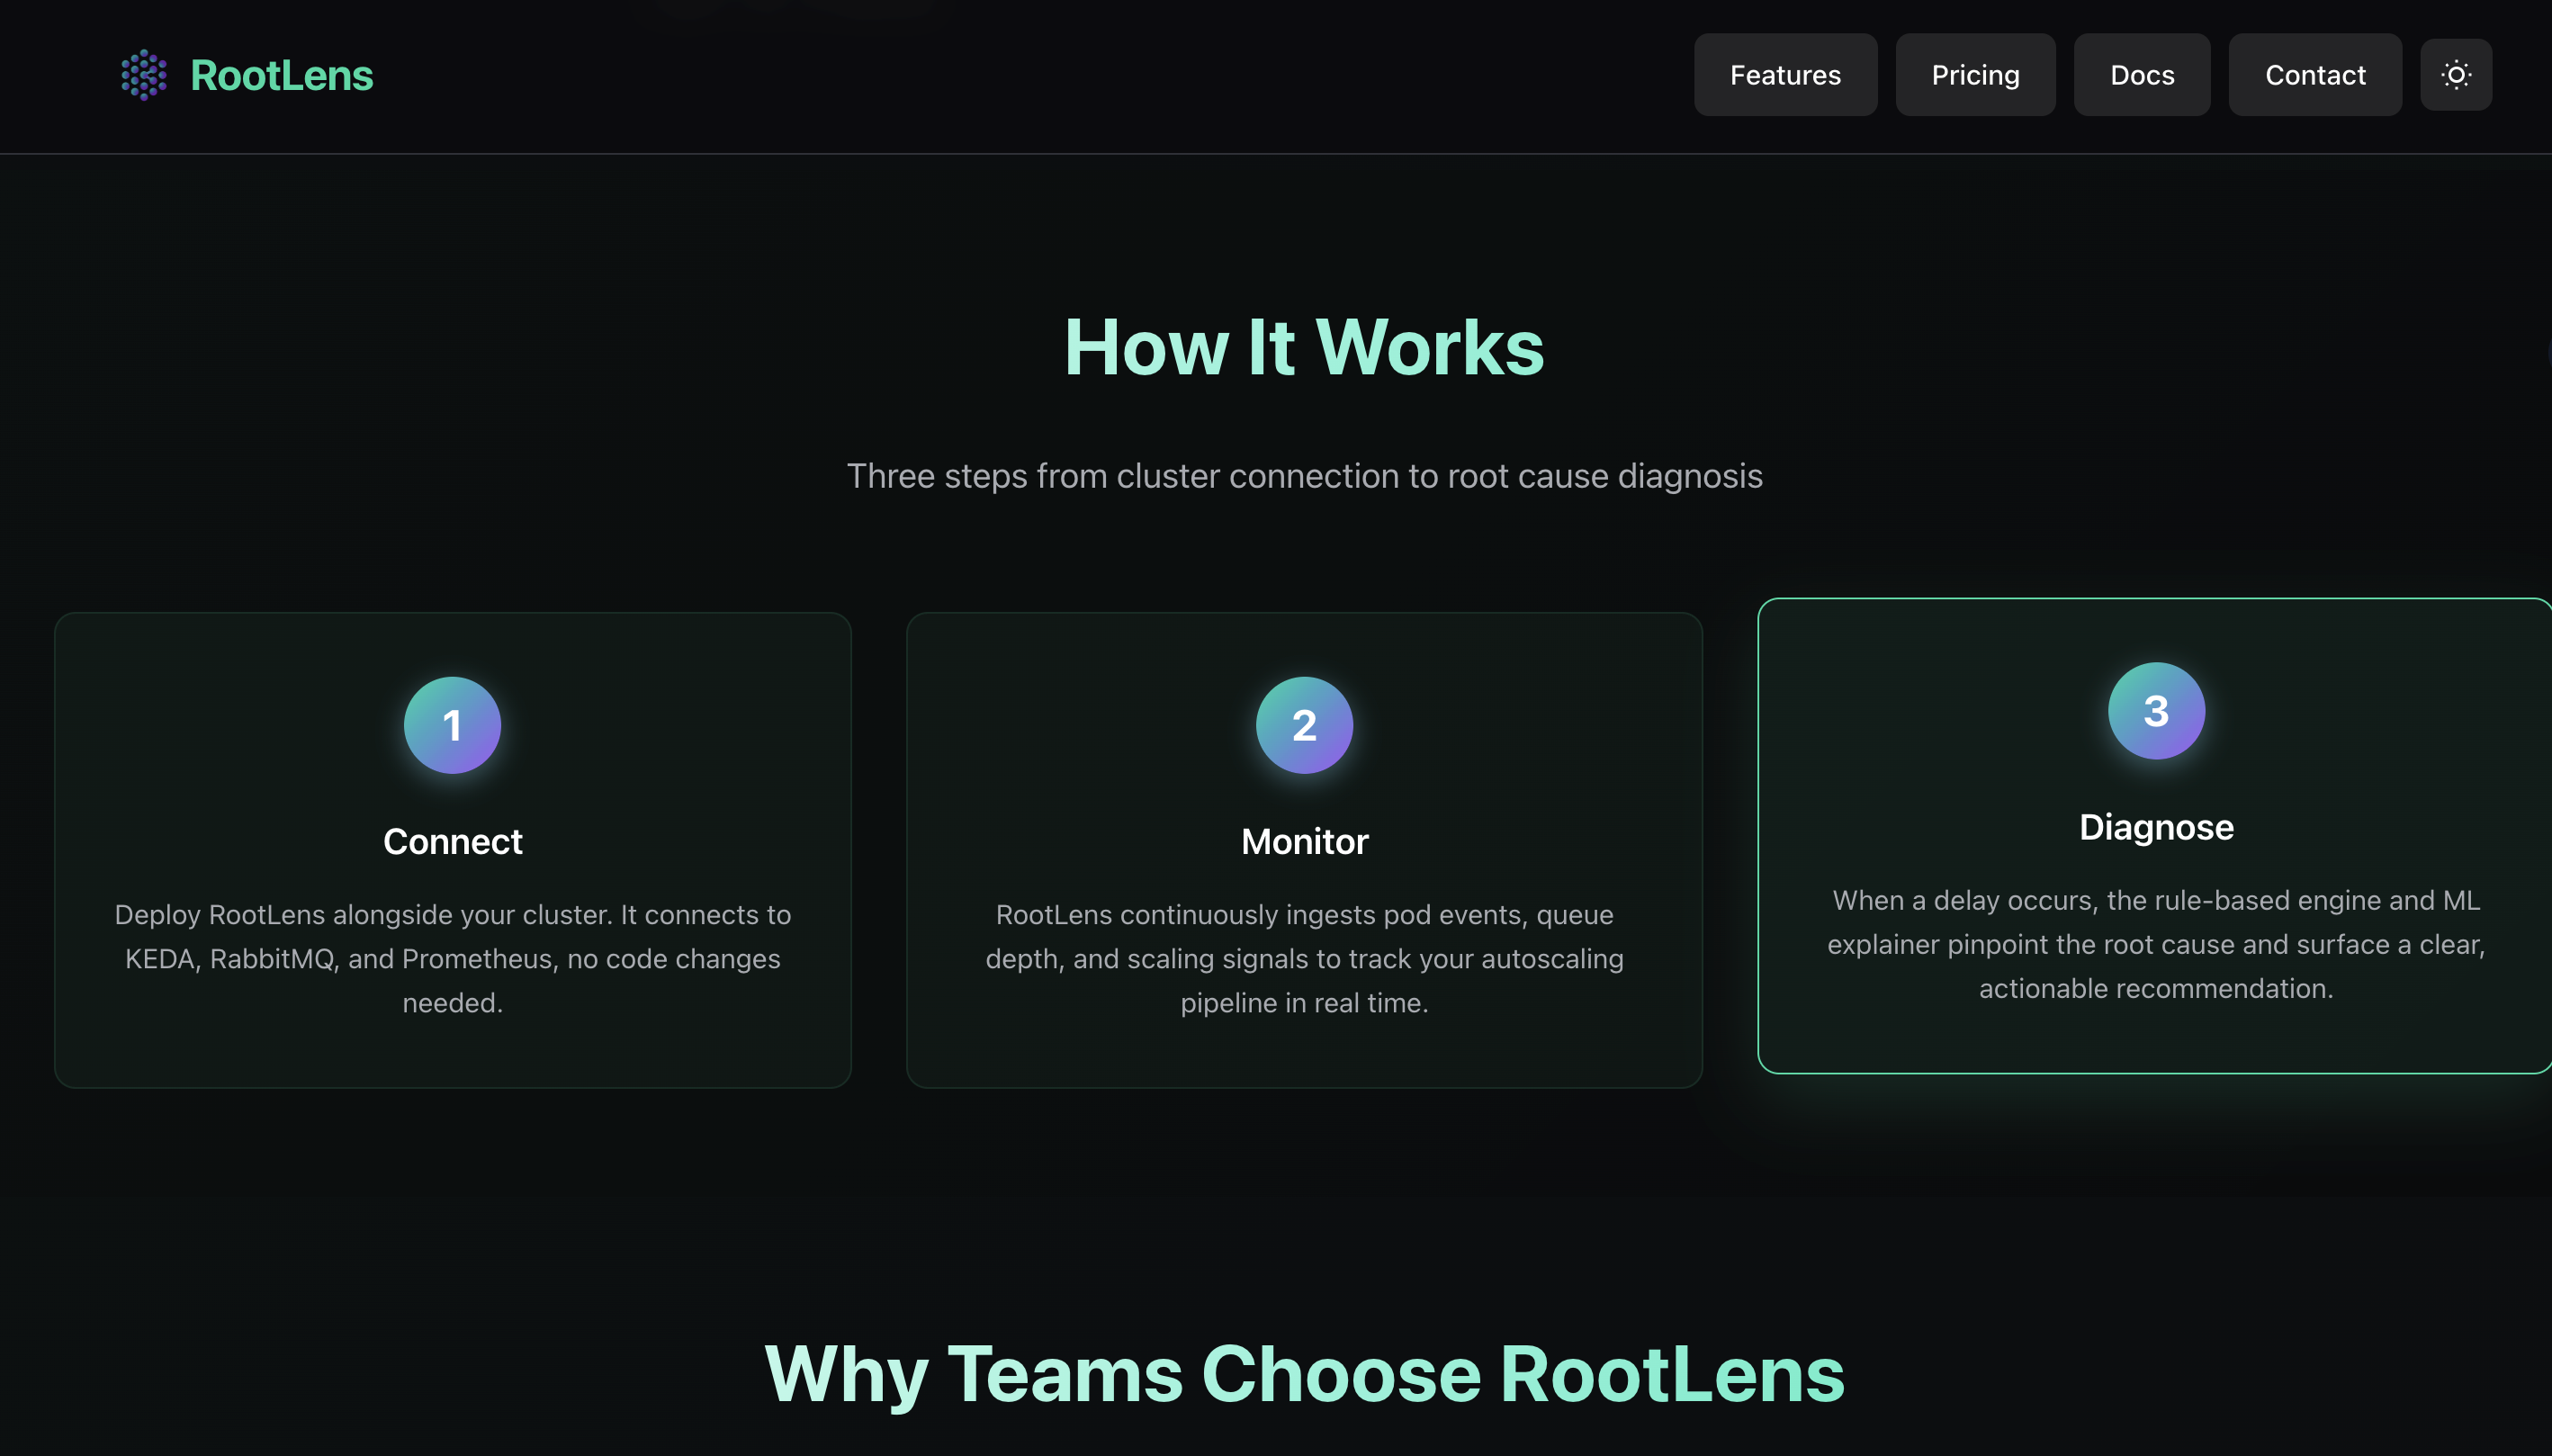
\includegraphics[width=\textwidth]{thesis/assets/main-4.png}
\caption{Marketing Website Page 4}
\label{fig:app_main4}
\end{figure}

\begin{figure}[H]
\centering
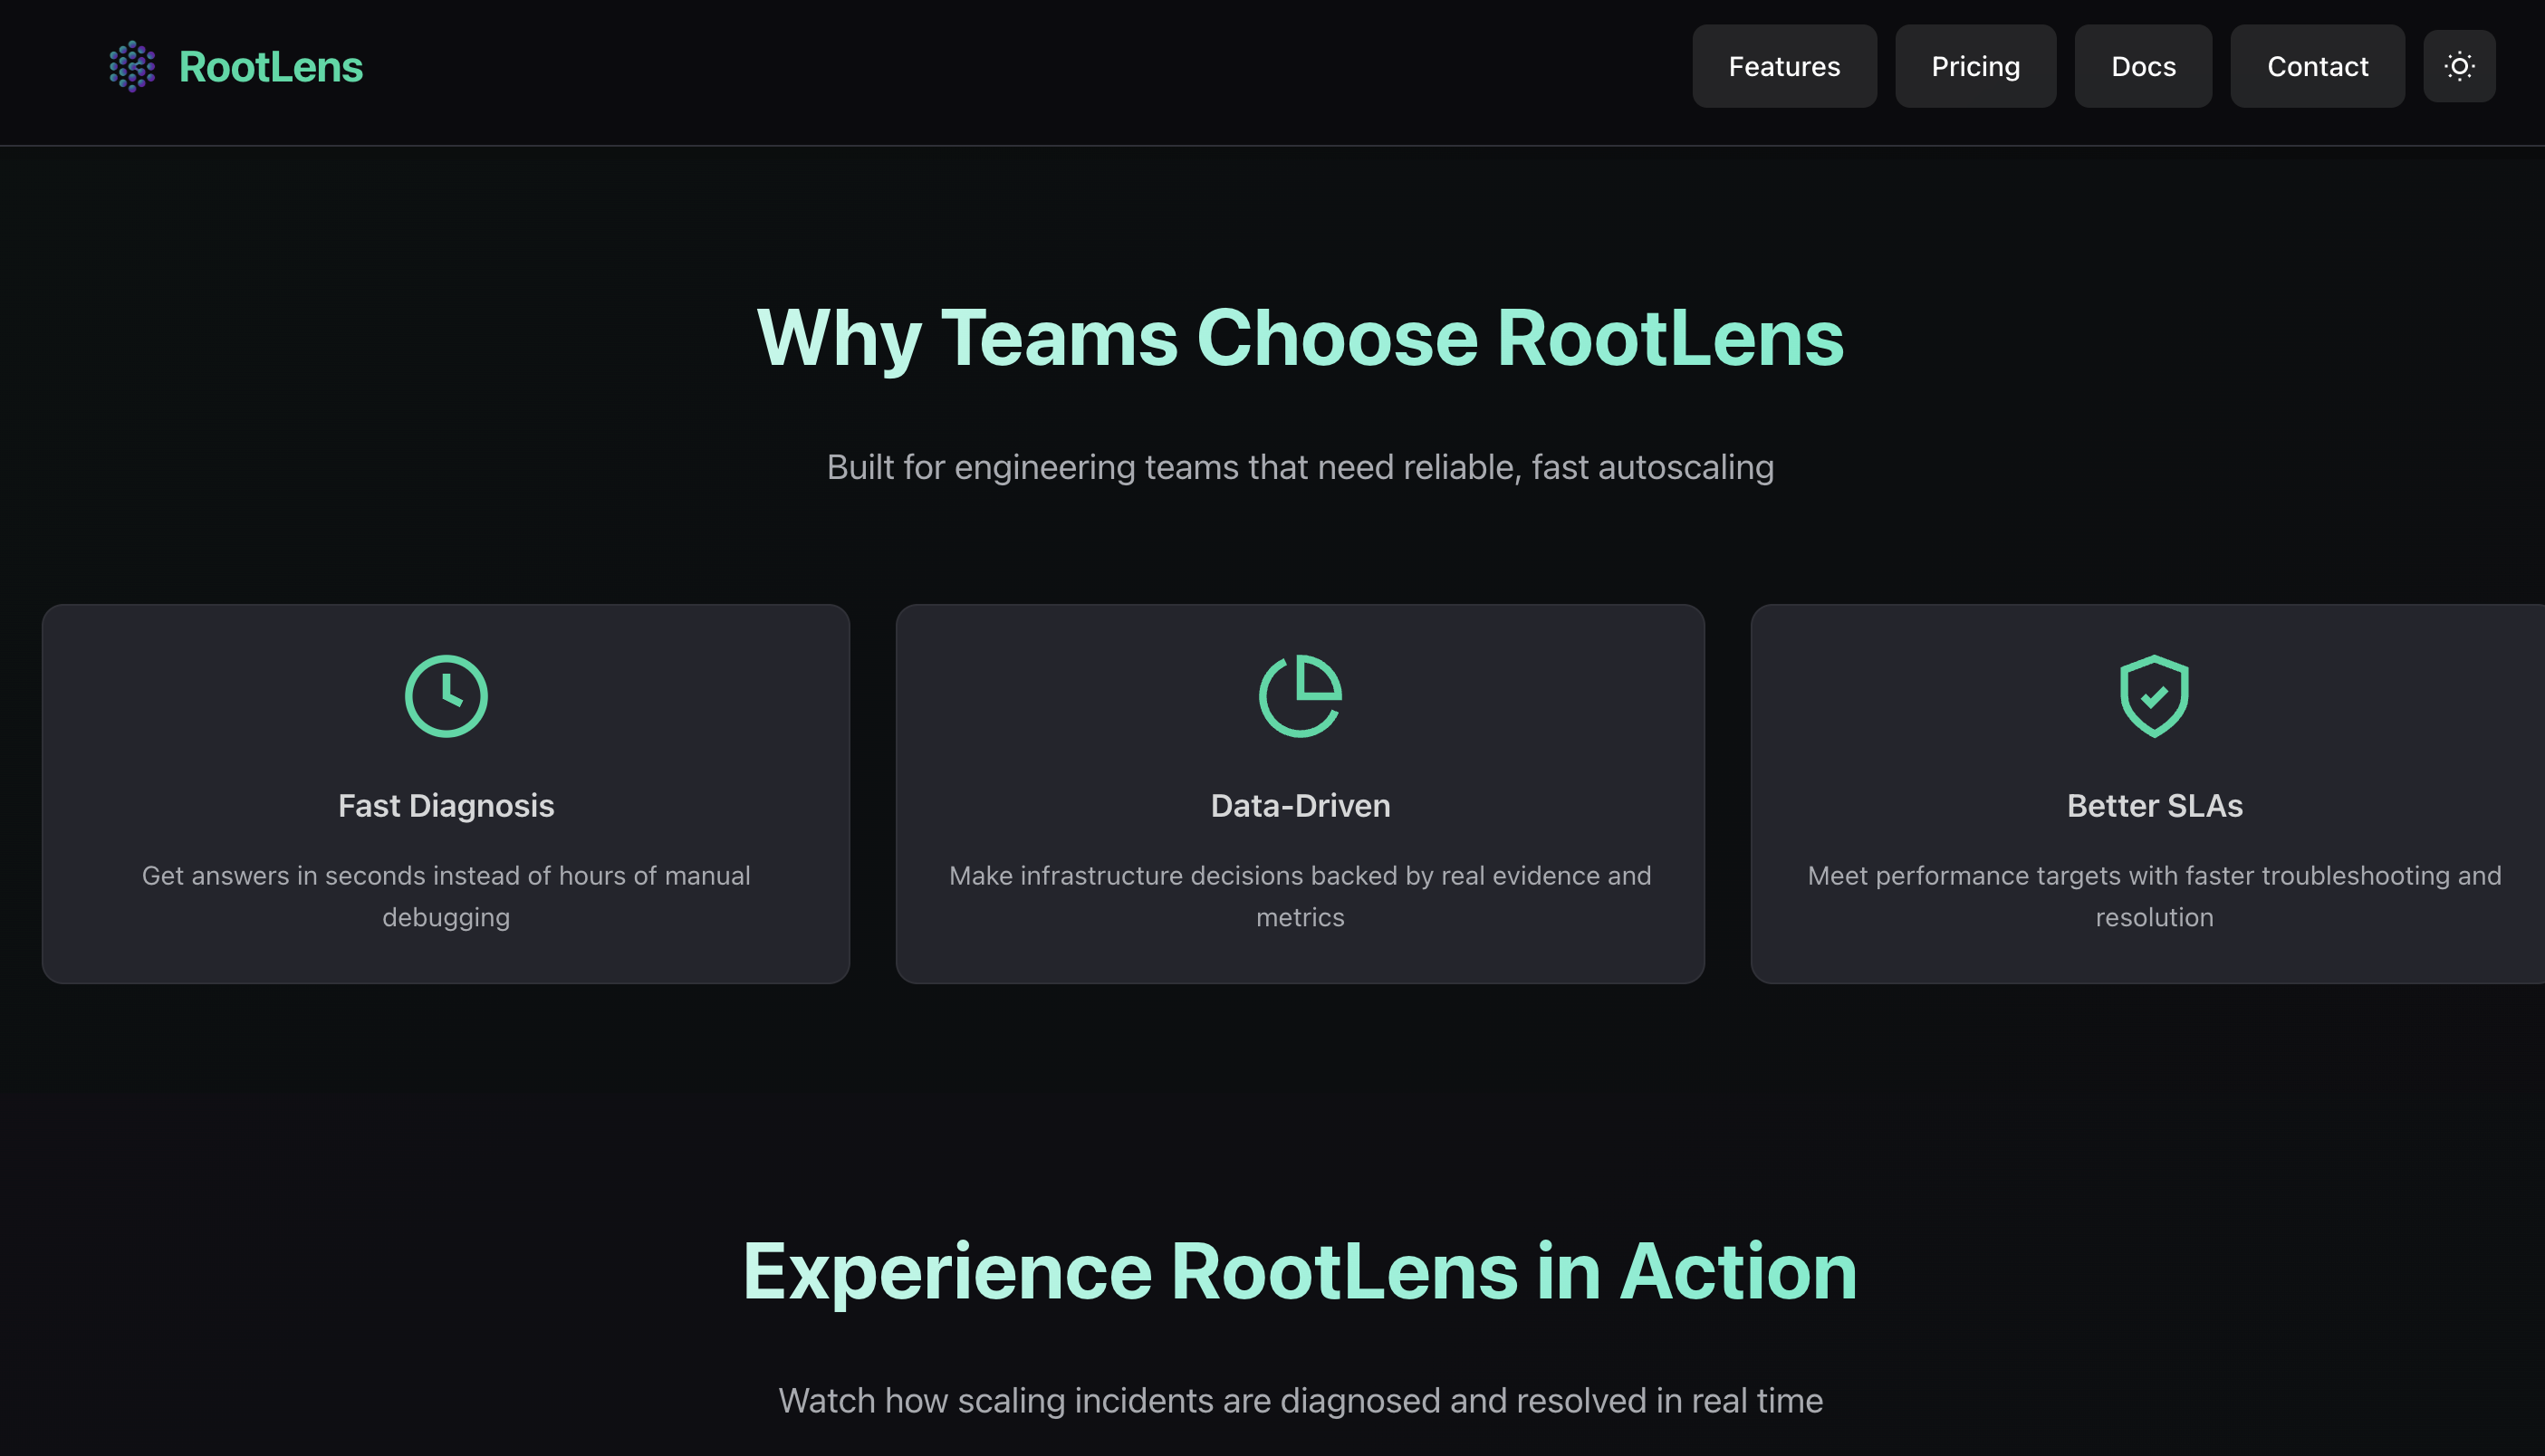
\includegraphics[width=\textwidth]{thesis/assets/main-5.png}
\caption{Marketing Website Page 5}
\label{fig:app_main5}
\end{figure}

\begin{figure}[H]
\centering
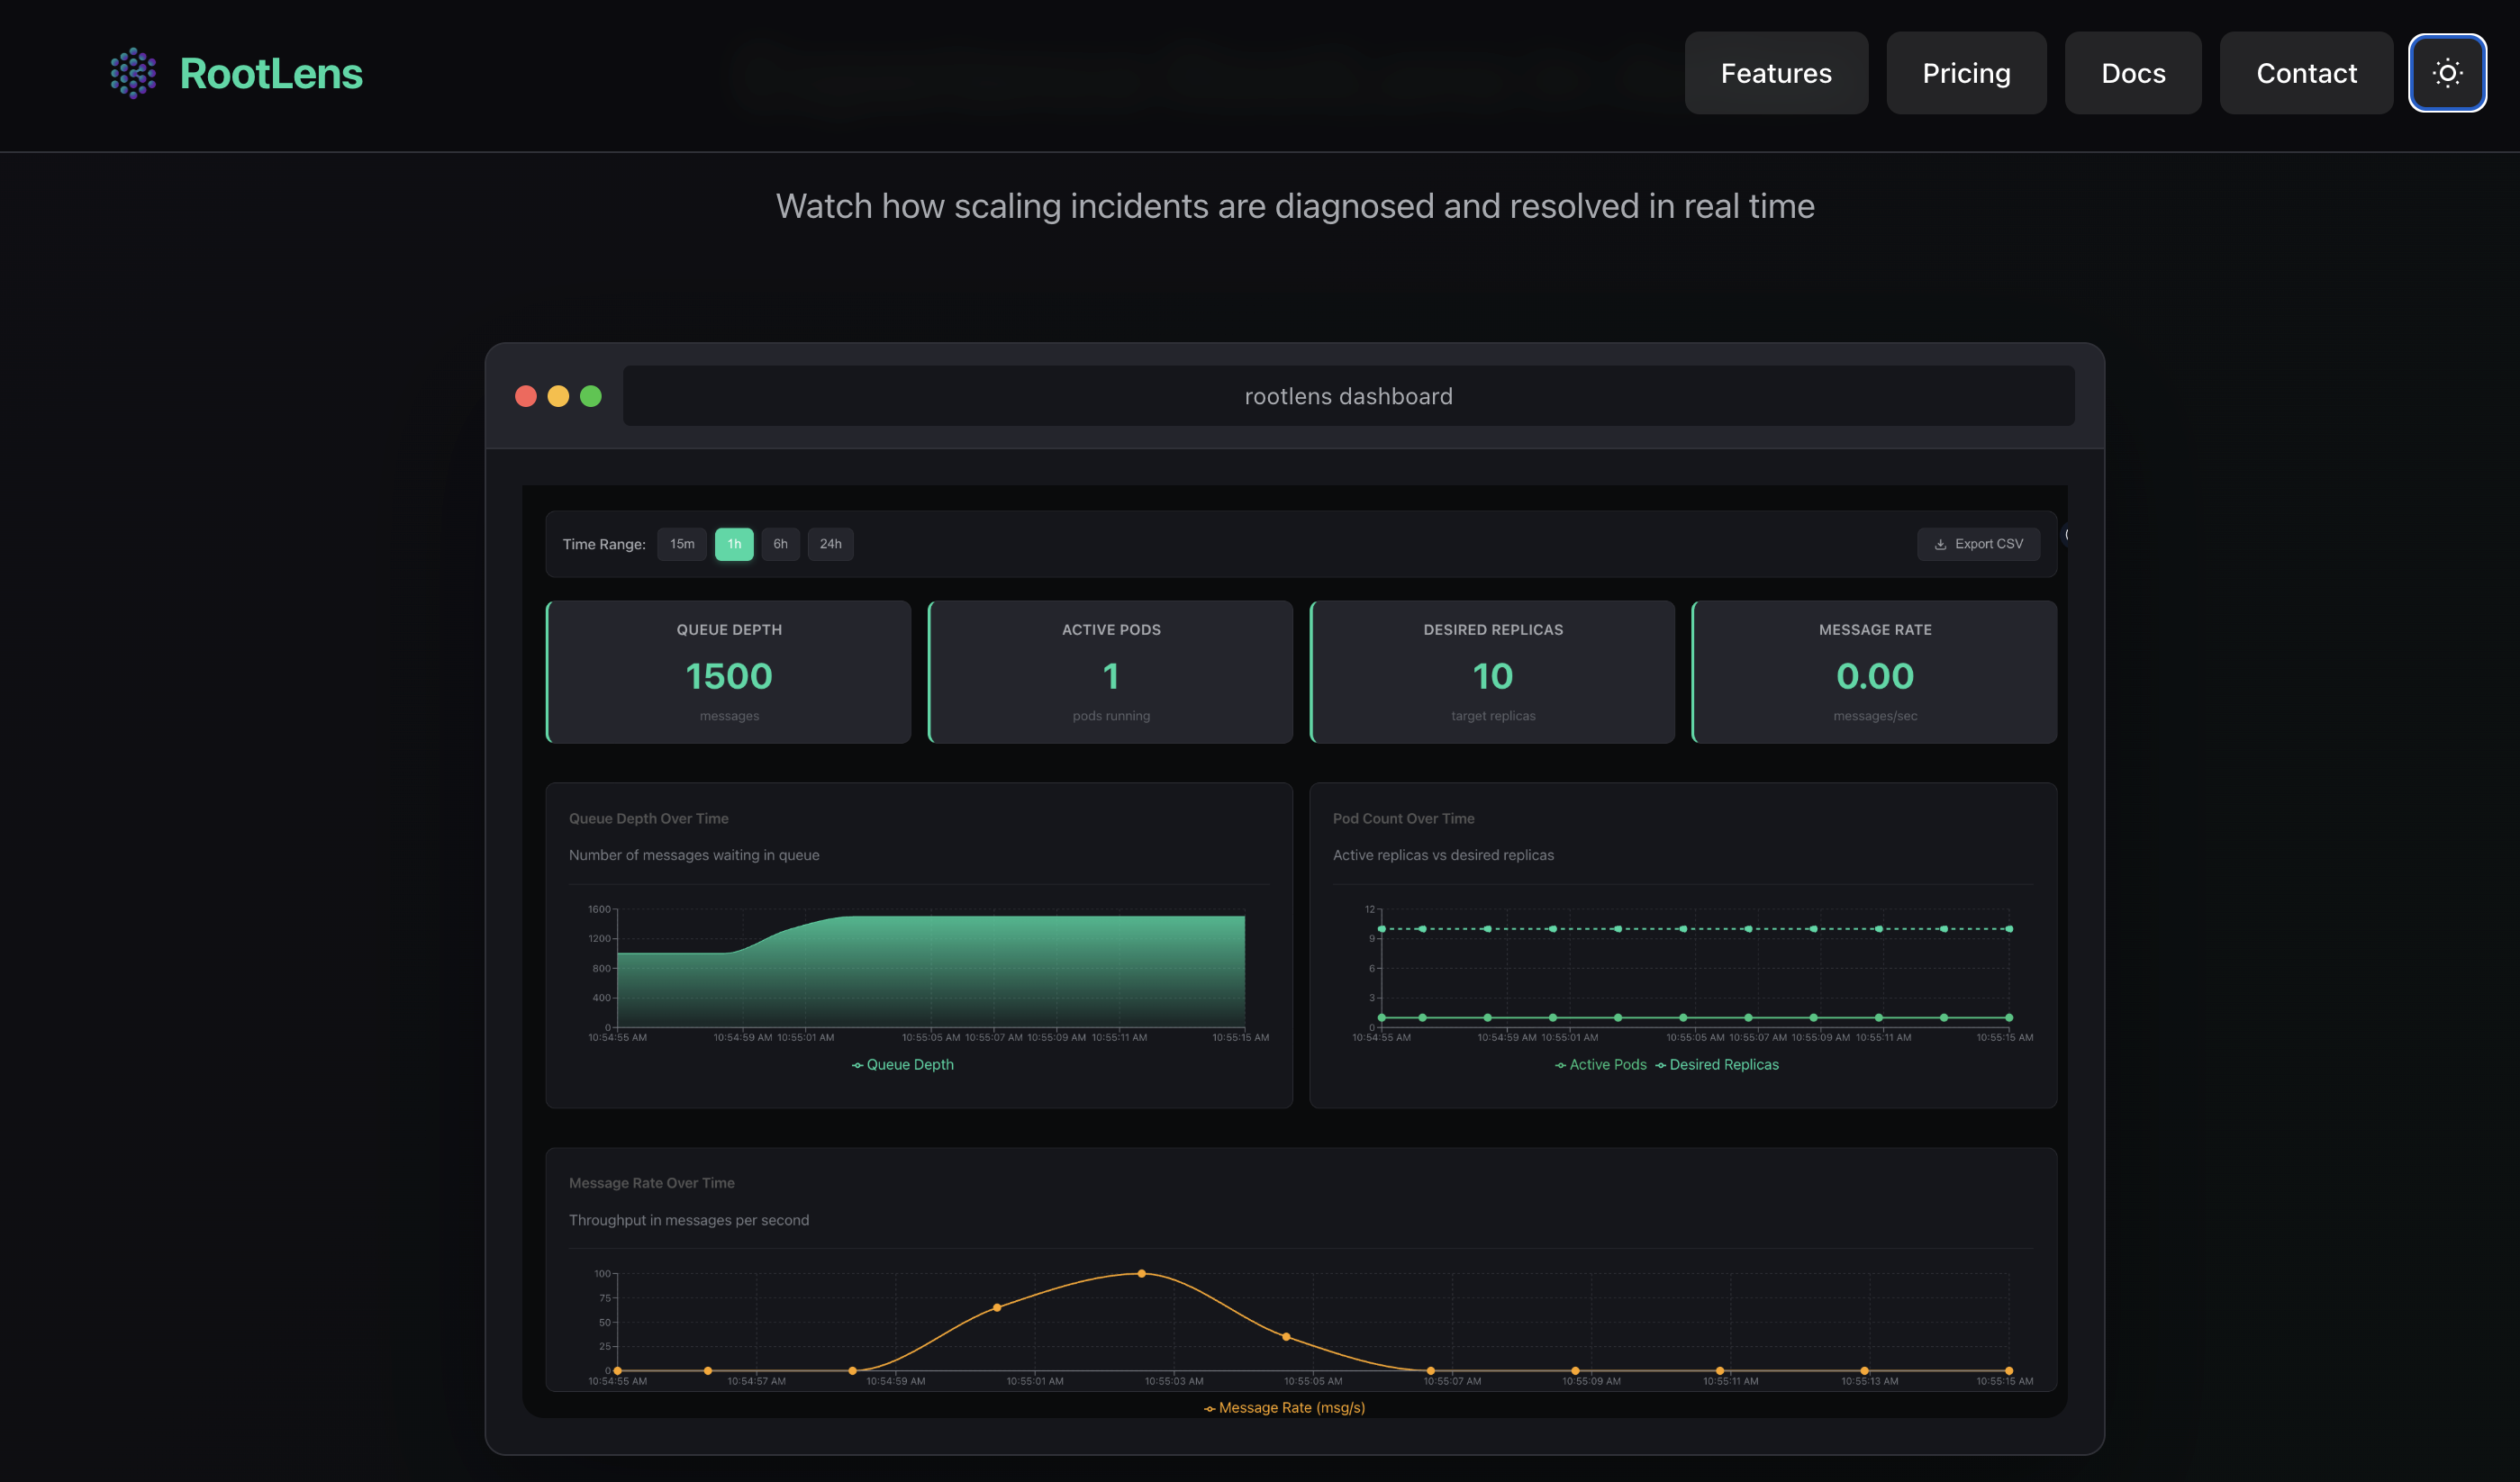
\includegraphics[width=\textwidth]{thesis/assets/main-6.png}
\caption{Marketing Website Page 6}
\label{fig:app_main6}
\end{figure}

\begin{figure}[H]
\centering
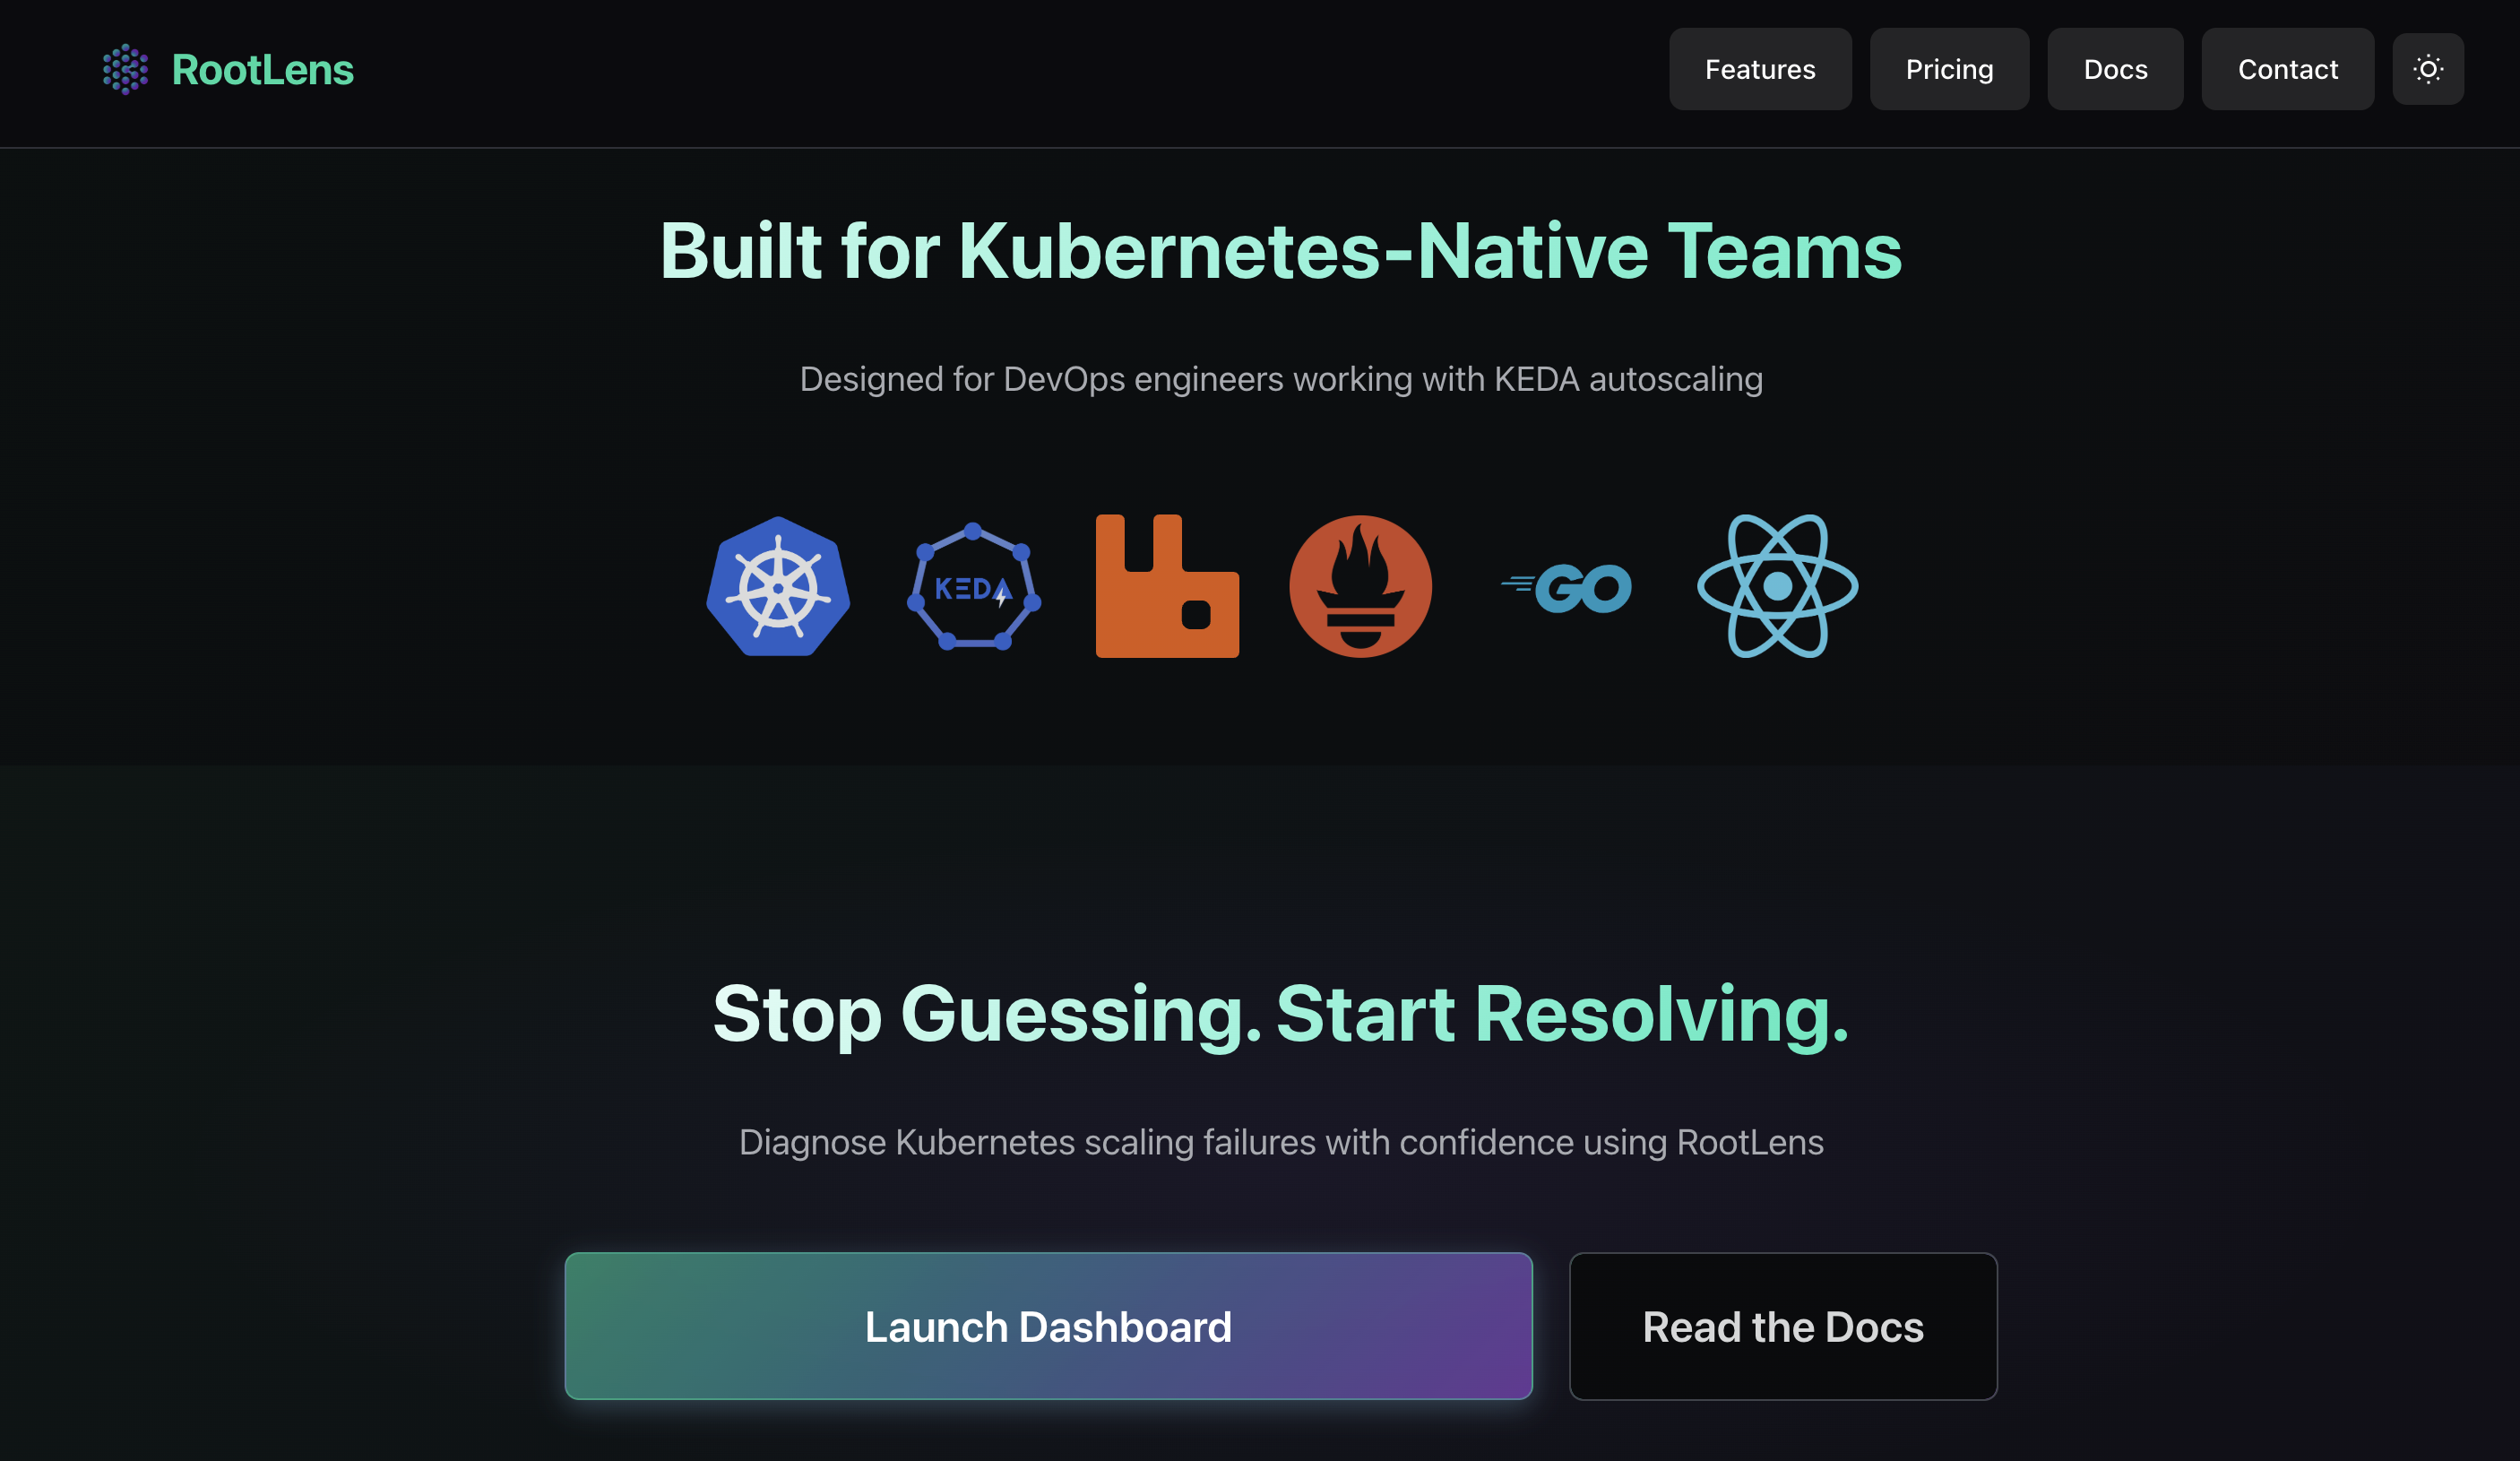
\includegraphics[width=\textwidth]{thesis/assets/main-7.png}
\caption{Marketing Website Page 7}
\label{fig:app_main7}
\end{figure}

% ==========================

\section*{Appendix E: Other Materials}
\addcontentsline{toc}{section}{Appendix E: Other Materials}
\label{appendix:evaluation_materials}

\begin{figure}[H]
\centering
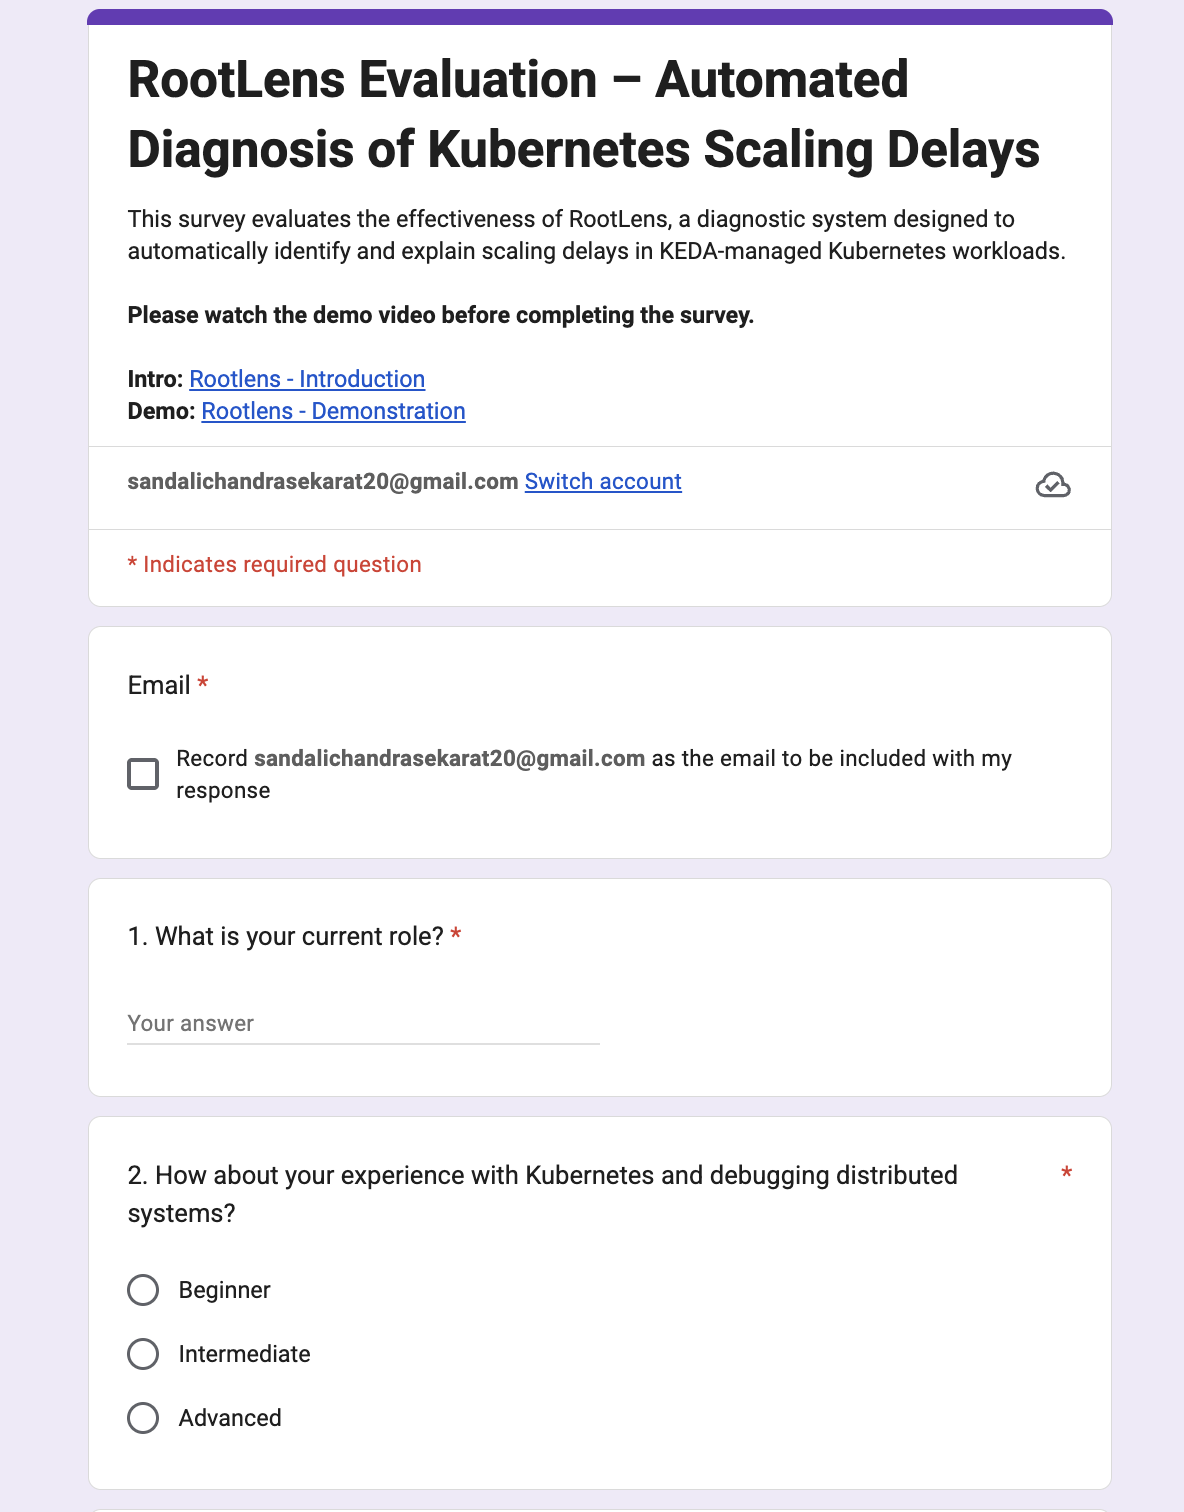
\includegraphics[width=\textwidth]{thesis/assets/google_form.png}
\caption{Shared Google Form for Evaluations}
\label{fig:google_form}
\end{figure}

\begin{figure}[H]
\centering
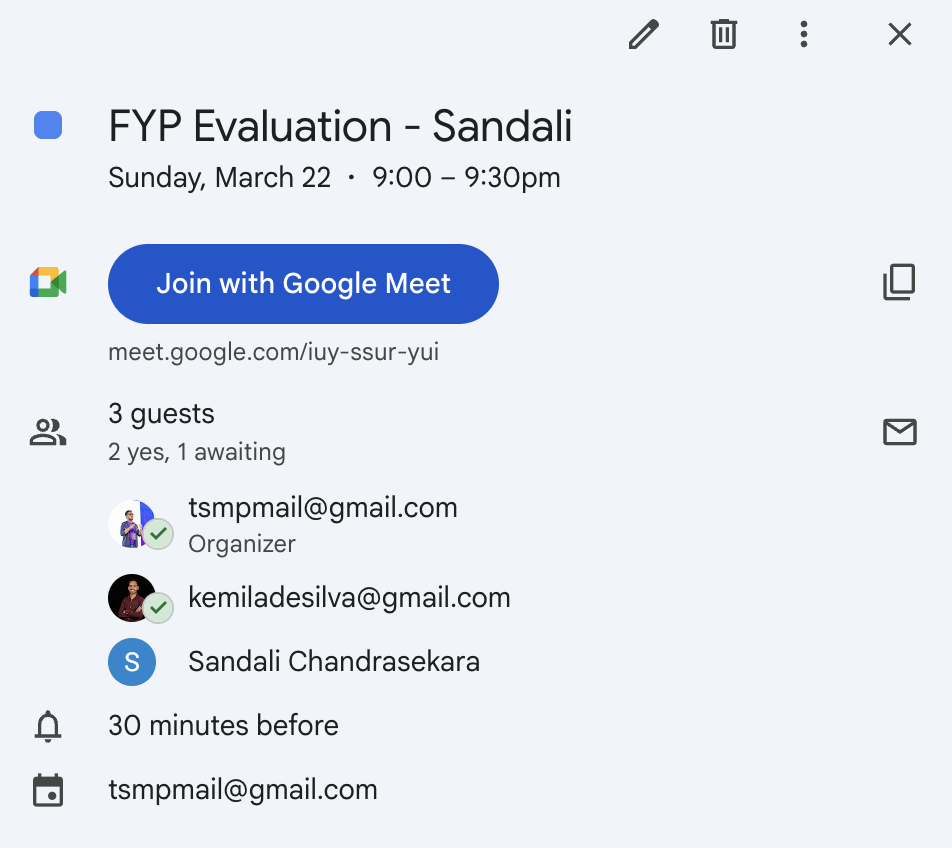
\includegraphics[width=\textwidth, height=0.4\textheight, keepaspectratio]{thesis/assets/eval_meeting.png}
\caption{Evaluation Meetings}
\label{fig:eval_meet}
\end{figure}

\begin{figure}[H]
\centering
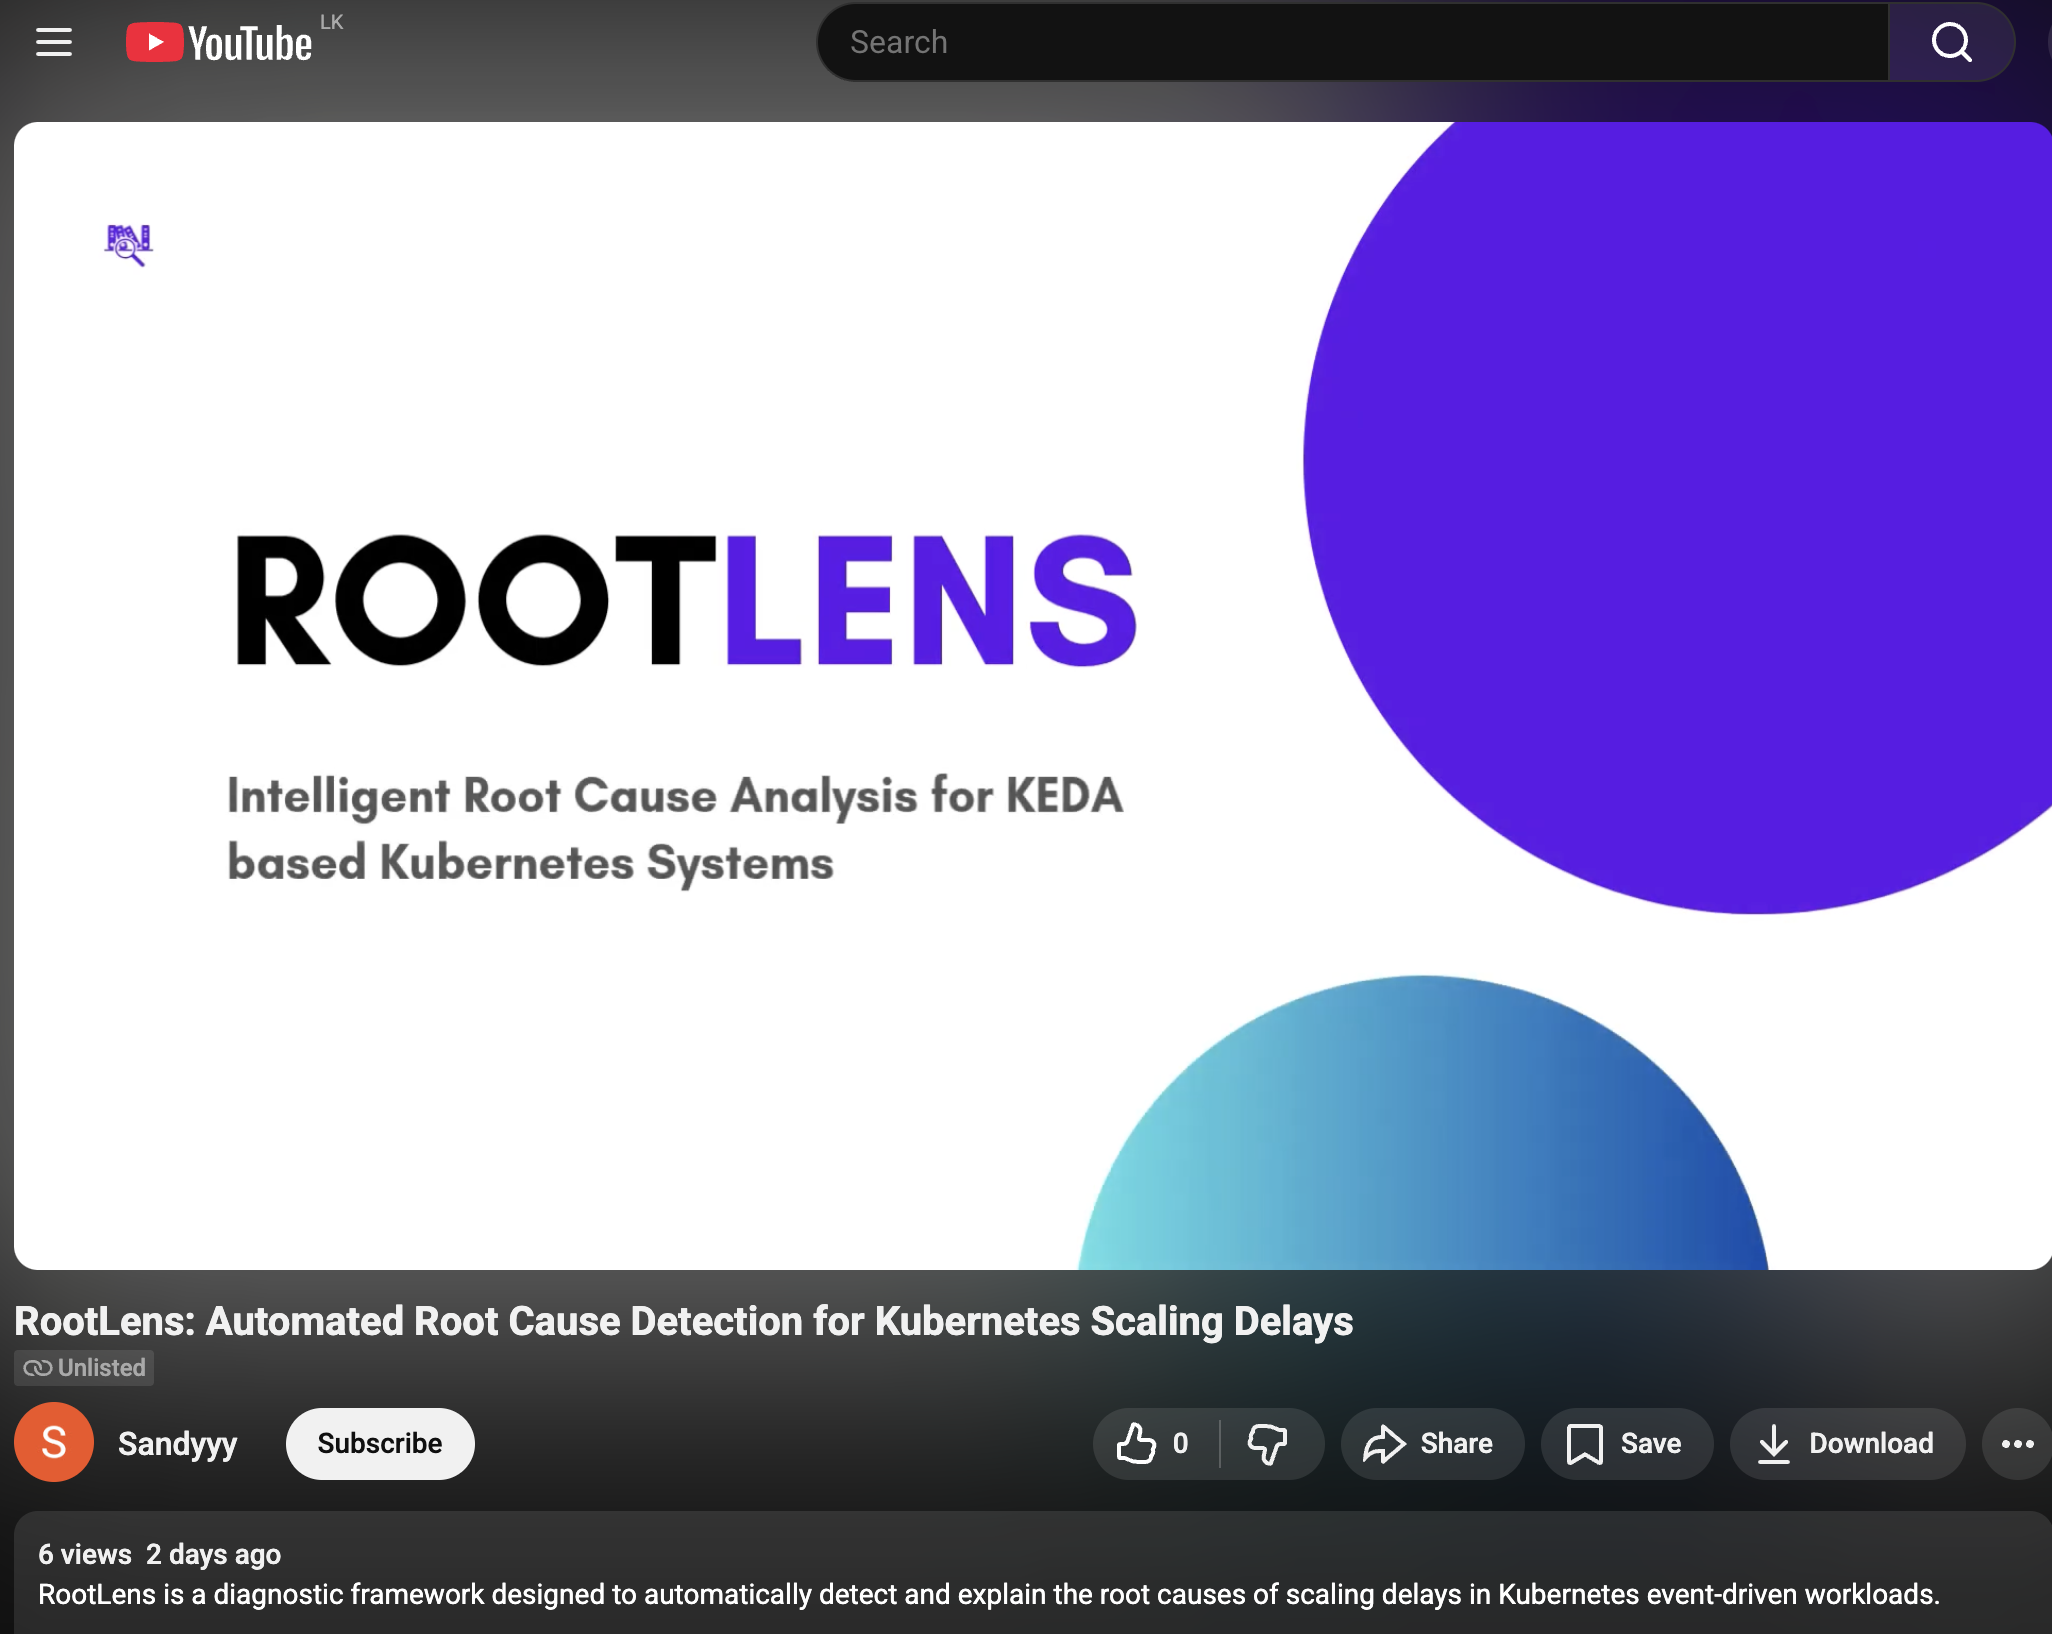
\includegraphics[width=\textwidth, height=0.4\textheight, keepaspectratio]{thesis/assets/intro_video.png}
\caption{Shared Introduction Video}
\label{fig:intro_video}
\end{figure}

\begin{figure}[H]
\centering
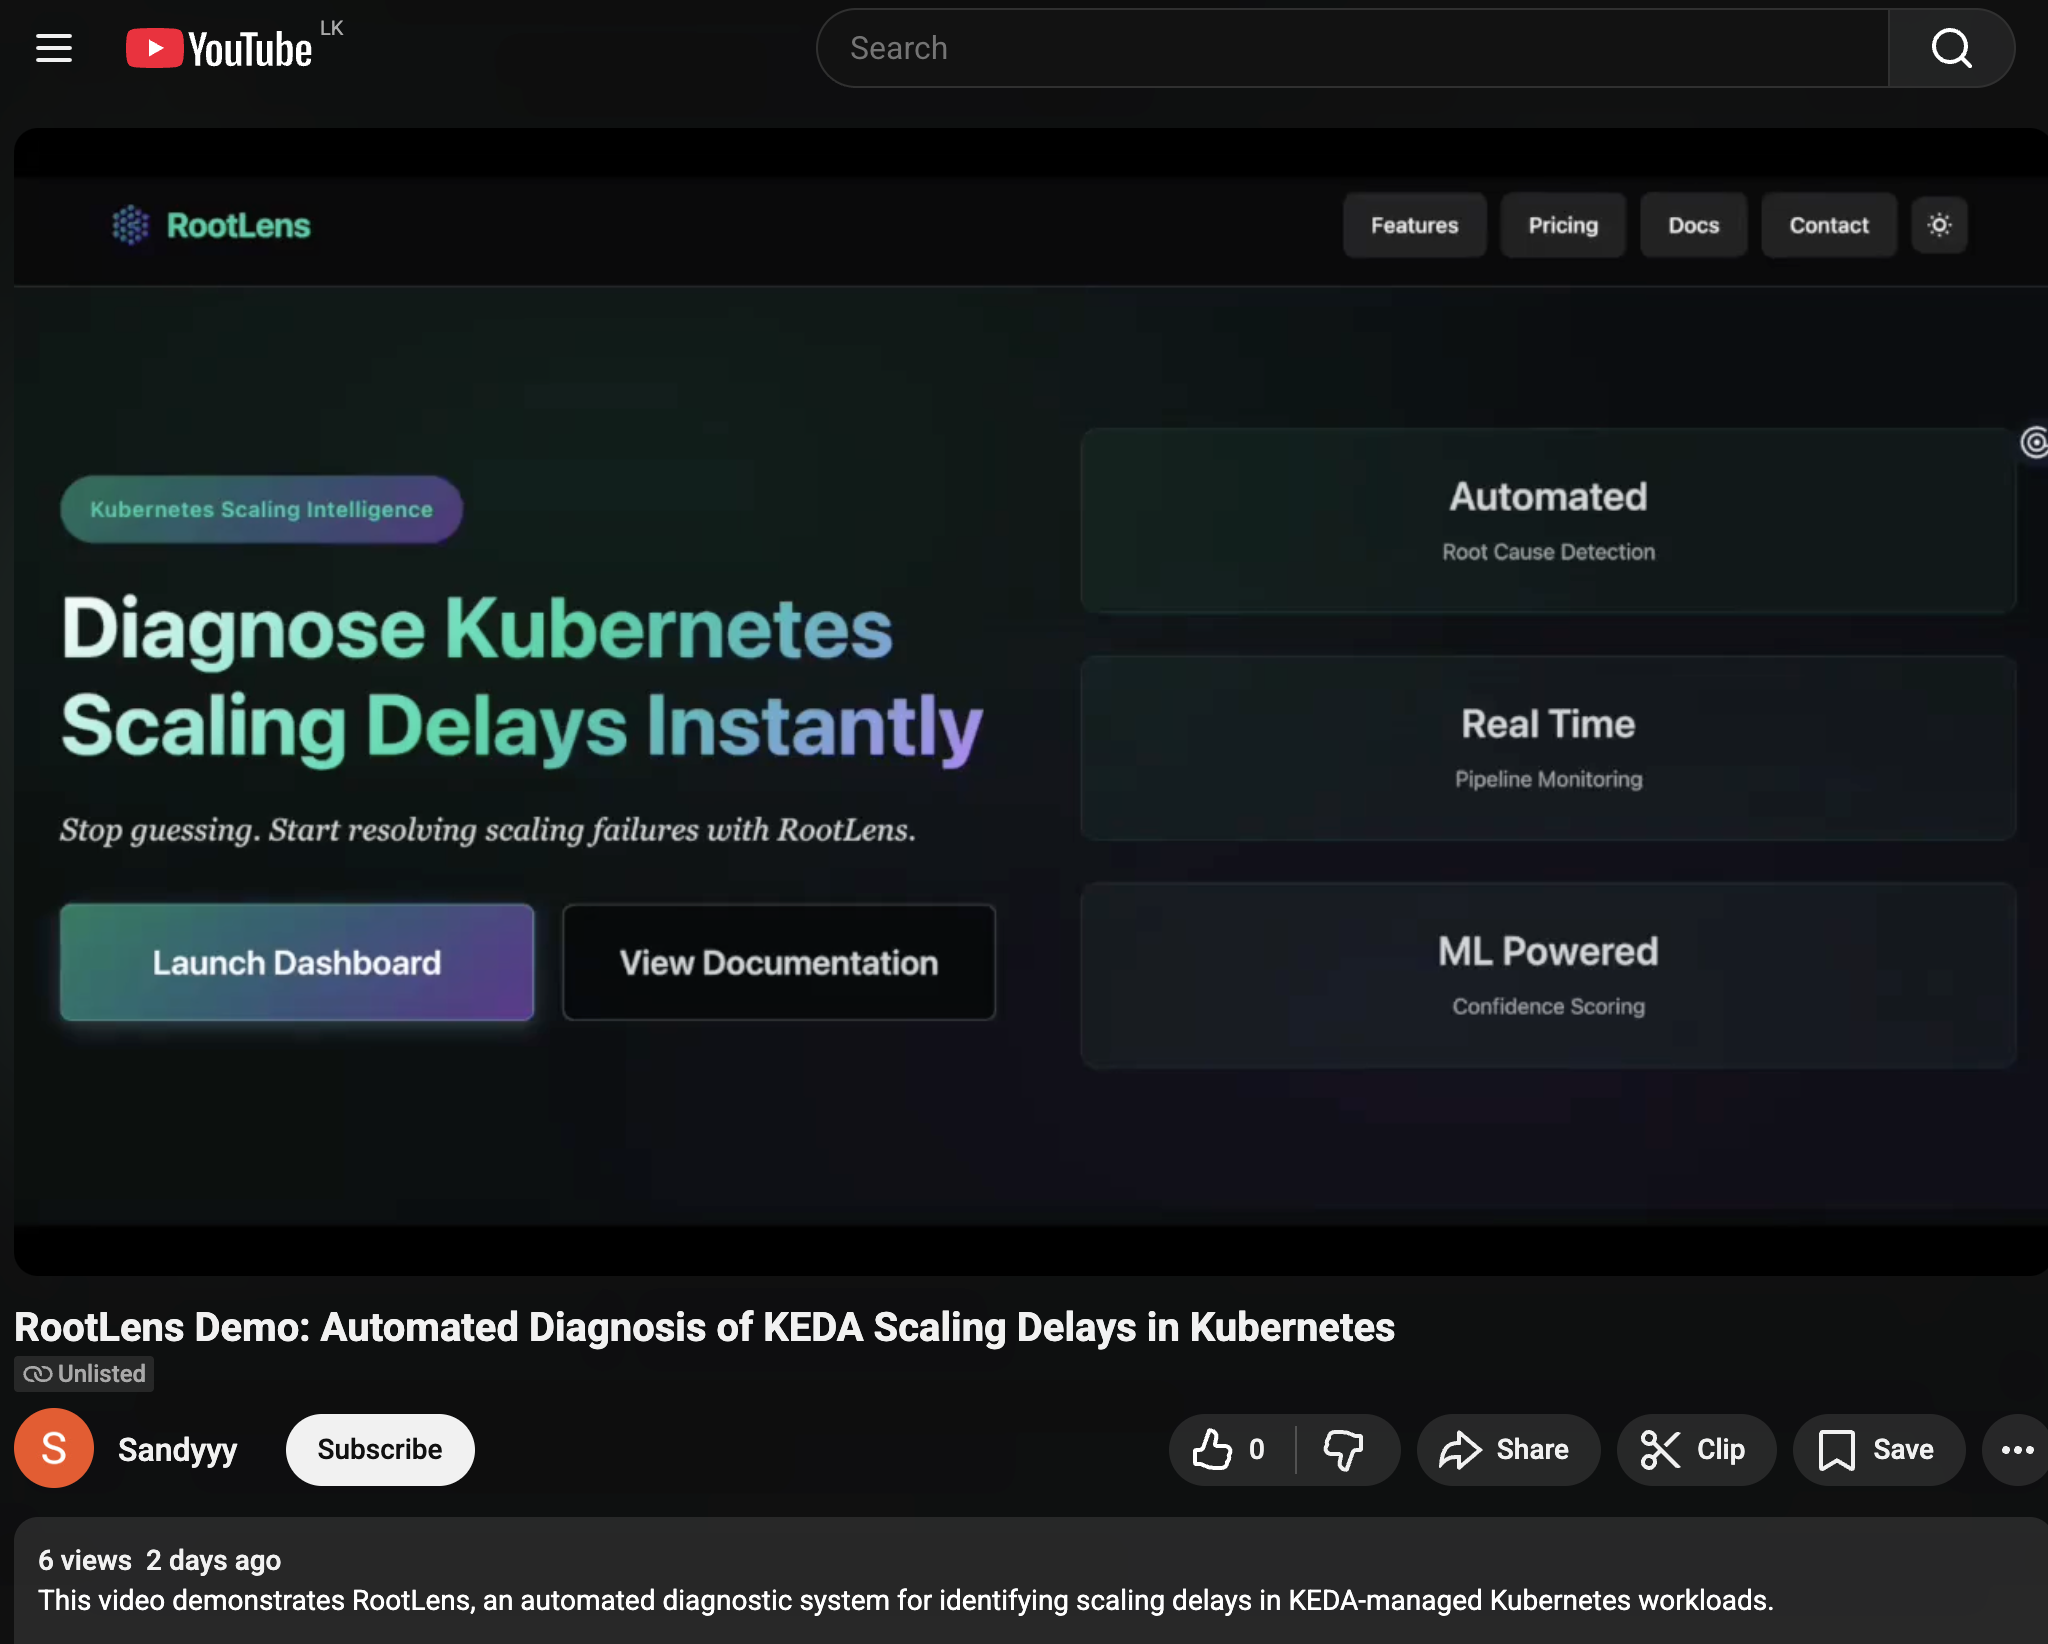
\includegraphics[width=\textwidth, height=0.4\textheight, keepaspectratio]{thesis/assets/demo_video.png}
\caption{Shared Demo Video}
\label{fig:demo_video}
\end{figure}



